%!TEX root = main.tex
\documentclass[11pt, a4paper, german]{scrartcl}

\usepackage[german]{babel}
\usepackage[utf8]{inputenc}

\usepackage{amsmath,amssymb}
\usepackage{amsthm}
\usepackage[arrow, matrix, curve]{xy}
\usepackage{easy-todo}

\usepackage{tikz}
%\usepackage{pgfplots}
%\usepackage{picinpar}
%\usepackage{cutwin}
\usepackage{tikz-3dplot}
\usepackage{graphicx}
\usepackage{float}
\usepackage{caption}
\usepackage{subcaption}
\usepackage{wrapfig}
\graphicspath{ {Images/} {../Images/}}
\usepackage{epstopdf}


\usepackage{BA_Titelseite}
\usepackage{topology}


%Namen des Verfassers der Arbeit
\authornew{Daniel Valenzuela}

%Geburtsdatum des Verfassers
\geburtsdatum{21.07.1992}
%Gebortsort des Verfassers
\geburtsort{München}
%Datum der Abgabe der Arbeit
\date{\today}

%Name des Betreuers
% z.B.: Prof. Dr. Peter Koepke
\betreuer{Betreuer: Prof. Dr. Ursula Hamenstädt}
%Name des Instituts an dem der Betreuer der Arbeit tätig ist.
%z.B.: Mathematisches Institut
\institut{Mathematisches Institut}
%Titel der Bachelorarbeit
\title{Alexander Norm and Thurston Norm}
%Do not change!
\ausarbeitungstyp{Bachelorarbeit Mathematik}



\begin{document}

\maketitle
\tableofcontents
%!TEX root = main.tex
\section{Einführung}
		
	\begin{minipage}[t][\textheight][t]{0.76\textwidth}

	Diese Arbeit beschäftigt sich mit der Verallgemeinerung von Knoten- und Verschlingungsinvarianten. Das Ziel ist die Ausarbeitung des Beweises von McMullens Ungleichung (2002), welche die bekannte Abschätzung $\Grad \Delta_K \leq g(K)$ aus der Knotentheorie für kompakte orientierte 3-Mannigfaltigkeiten deren Rand höchstens aus Tori besteht, verallgemeinert.

	Die Theorie der Knoten beschäftigt sich mit Äquivalenzklassen von Knoten und dem Finden von Invarianten solcher Äquivalenzklassen. In der differenzierbaren Kategorie bezeichnet man mit einem Knoten eine glatte orientierte Einbettung $S^1\into S^3$ und man definiert zwei Knoten als äquivalent, wenn ein orientierungserhaltener Diffeomorphismus $S^3\to S^3$ existiert, der beide Knoten ineinander überführt. Insbesondere entstehen in der differenzierbaren Kategorie keine exotischen Exemplare eines Knotens, die man als "`wild"' bezeichnet. Als häufig betrachtete Invariante hat sich die orientierte Diffeomorphieklasse der kompakten 3-Mannigfaltigkeit ergeben, die man das Knotenkomplement nennt. Dieses entsteht durch Entnehmen einer offenen Tubenumgebung des eingebetteten Knotens $S^1 \into S^3$ und ist eine naheliegende Knoteninvariante. Letzteres bedeutet: Äquivalente Knoten haben diffeomorphe Knotenkomplemente durch einen orientierungserhaltenden Diffeomorphismus. Häufig stellen sich Knoteninvarianten lediglich als Invarianten der Knotenkomplemente heraus; etwa bezeichnet man mit der Gruppe eines Knotens die Fundamentalgruppe des Komplements. Um die Qualität und Feinheit dieser aus dem Komplement entstehenden Invarianten zu beurteilen, ist es zunächst wichtig jene des Knotenkomplements zu beurteilen. Es gibt unzählige Ergebnisse, die aus Berechnungen auf dem Knotenkomplement entstehen, woraus sich die Relevanz dieser Frage ableitet. Tatsächlich zeigen Gordon und Luecke in~\cite[1989]{Gordon.1989} die Umkehrung, dass orientiert diffeomorphe 3-Mannigfaltigkeiten die aus Knotenkomplementen entstehen, aus äquivalenten Knoten entstehen. Es handelt sich bei dem Knotenkomplement also um eine vollständige Knoteninvariante. 

	Diese Arbeit nimmt solche Invarianten, die aus Knotenkomplementen hervorgehen, als Ausgangspunkt.


	\vfill
	\begin{minipage}[t]{0.7\textwidth}
		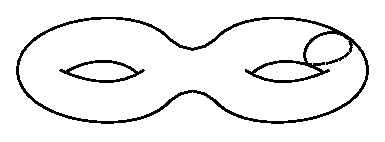
\includegraphics{zyklbott} 
	\end{minipage}
	\begin{minipage}[t]{0.2\textwidth}
	\vspace{-1cm}
	\huge$\longleftarrow$
	\vfill

	\end{minipage}
	\vspace{.63cm}
		\captionof{figure}{Unendlich zyklische Überlagerung} \label{fig:zykl}
	\end{minipage}
	\hfill
	\begin{minipage}[t]{0.2\textwidth}
	\vfill \begin{flushright}
		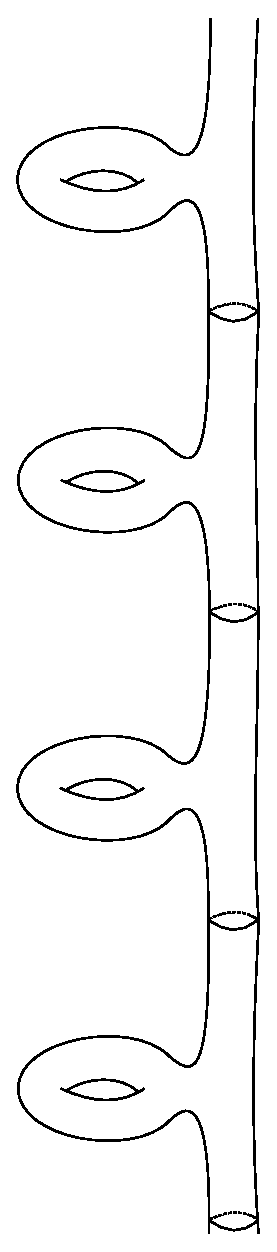
\includegraphics{zyklright} 
	\end{flushright}
	\end{minipage}

	Alexander definiert 1928 eine topologische Invariante des Knotenkomplements (vgl.\,\cite{Alexander.1928}), die einem Knotenkomplement eine Klasse von Laurentpolynomen mit eindeutigem Grad zuordnet. Im Jahr 1934 stellt Seifert in seiner Arbeit "`Geschlecht von Knoten"'~\cite{Seifert.1934} mit dem Knotengeschlecht eine Invariante vor, welche die minimale Komplexität einer orientierten eingebetteten Fläche berechnet, die den Knoten aufspannt (nach der Klassifikation von Flächen wird diese in Termen des Geschlechts gemessen). Weiter gibt er darin eine explizite Konstruktion für die Existenz solcher Flächen an, die sogenannte Seifert-Konstruktion. Dieses Knotengeschlecht liefert die Möglichkeit jeden Knoten von dem Unknoten zu unterscheiden. Das bedeutet, dass nur nur der Unknoten aus dem Rand einer eingebetteten Scheibe hervorgeht. Natürlich liefert die Seifert-Konstruktion eine Fläche mit einem gewissen Geschlecht. Es ist jedoch ein deutlich komplizierteres Unterfangen, wenn man zeigen möchte, dass eine gefundene Fläche in ihrer Komplexität nicht unterboten werden kann. Entsprechend günstig erweist sich Seiferts Resultat, dass der Grad des Alexander-Polynoms eines Knotens eine untere Schranke für sein Geschlecht definiert. Hat man also eine eingebettete orientierte Seifert-Fläche eines Knotens gefunden, von der man vermutet minimales Geschlecht zu haben, so kann man den Grad des Alexander-Polynoms zu dem Knoten berechnen und verifiziert in manchen Fällen die Vermutung.

	Der wesentliche Gegenstand dieser Arbeit ist die Verallgemeinerung dieser beiden auf Knotenkomplementen definierten Invarianten, zu Invarianten auf kompakten, orientierbaren 3-Mannigfaltigkeiten mit Rand, der maximal aus Tori besteht. Für diese Invarianten stellt McMullen in~\cite{MCMULLEN.2002} fest, dass sich auch die oben erwähnte Abschätzung aus der Knotentheorie verallgemeinern lässt. Diese Arbeit beschäftigt sich mit diesem Resultat, welches dieser Arbeit als Haupttheorem~\ref{thm:haupttheorem} zugrunde liegt.

	Um dem Leser den Einstieg in die Arbeit möglichst angenehm zu gestalten, sei im Folgenden noch die Art der Verallgemeinerungen und der Aufbau der Arbeit skizziert.

    Im Falle eines Knotens berechnet sich die erste Kohomologie des Komplementes zu einer freien abelschen Gruppe von Rang 1. Die orientierte Seifert-Fläche (welche den Knoten aufspannt) lässt sich als Homologieklasse auffassen, vgl.\,Bemerkung~\ref{bem:untermannigfaltigkeitenalshomologie}. Als solche ist sie Lefschetz dual zu einem $\phi$ der ersten Kohomologie. Nun stellt man fest, dass die beiden betrachteten Knoteninvarianten, sich als Invarianten der Kohomologie auffassen lassen. So verallgemeinert die Alexander-Norm auf der ersten Kohomologie den Grad des Alexander-Polynoms von $\phi$, vgl.\,Kapitel~\ref{sec:links}. Und die Thurston-Norm einer Kohomologieklasse berechnet die minimale Komplexität aller zu $\phi$ dualen, orientierten, eingebetteten Flächen. Sie verallgemeinert also das Knotengeschlecht, da sie sich im Falle eines Knotens aus einer geschlechtsminimierende Seifert-Fläche berechnet.

    Es stellt sich heraus, dass alle betrachteten Invarianten eine enge Beziehung zu unendlich zyklischen Überlagerungen haben. Diese können etwa durch Aufschneiden und Verkleben an einer zusammenhängenden 1-kodimensionalen Untermannigfaltigkeit gewonnen werden, siehe zum Beispiel Abbildung~\ref{fig:zykl}. Diese Abbildung ist für die Intuition und das Verständnis erheblich --- man könnte dem Leser fast raten, vor und nach jedem Kapitel die Abbildung~\ref{fig:zykl} zu betrachten und immer wieder neu zu reflektieren. Man beachte die Kompaktheit der Mannigfaltigkeit, wohingegen die Überlagerung unendlich erzeugte Homologie hat.

    Der Aufbau der Arbeit lässt sich wie folgt beschreiben: Das erste Kapitel bereitet das nötige algebraische und topologische Werkzeug für die Definitionen und Berechnungen der verallgemeinerten Invarianten vor. Weiter beschreibt es Konstruktionen, die in späteren Beweisen zielführend sein werden. Das nächste Kapitel definiert die Thurston-Norm eines Elementes $\phi \in H^1(M;\ZZ)$ und beweist eine Abschätzung gegen $b_1(\ker\phi)$. Anschließend präsentiert das Kapitel~\ref{sec:alexdefs} die Alexander-Norm und widmet dieser eine ausführliche algebraische Betrachtung. Weiter stellt es einen Zusammenhang der Alexander-Norm mit $b_1(\ker\phi)$ her. Diese Ergebnisse liefern den Beweis des Theorems, der mit einer Reihe von Modifikationen und Ergänzungen an die Beweisführung aus~\cite{MCMULLEN.2002} angelehnt ist. Das letzte Kapitel stellt weiterführende Fragen und gibt einige Anwendungen und Beispiele für Berechnungen an.   

    Bevor nun das Haupttheorem der Arbeit angegeben wird, möchte ich mich ausdrücklich bei meiner Betreuerin Prof. Ursula Hamenstädt bedanken. Nicht nur für die Wahl des interessanten Themas, sondern vor allem auch für die qualitative Betreuung und den hohen Zeit- und Geduldaufwand, den sie dafür eingebracht hat. Die gemeinsamen Diskussionen hatten eine extrem hohe Lerndichte für mich und das Wissen, dass ich im Rahmen der Bachelorarbeit gewonnen habe, geht weit über das Niedergeschriebene hinaus. Weiter möchte ich Prof. Matthias Kreck danken, dessen exzellente Vorlesung über die Differentialtopologie meine Intuition und Geschicklichkeit in differentialtopologischen Betrachtungen geprägt hat und mir einen guten Einstieg in diese Bachelorarbeit ermöglicht hat.
    %in diesem Rahmen?
\vfill
    \begin{thm}[McMullen]
    \label{thm:haupttheorem}
    	Sei $M$ eine kompakte, zusammenhängende, orientierbare Mannigfaltigkeit der Dimension 3. Falls der Rand dieser Mannigfaltigkeit nicht leer ist, so soll er aus einer Kollektion von Tori bestehen. Dann gilt folgende Abschätzung für die Alexander-Norm und die Thurston-Norm $\alex \cdot ,\thur \cdot : H^1(M;\ZZ) \to \RR$ der 3-Mannigfaltigkeit:
    	\[
    		\alex \phi \leq 
    		\begin{cases}
    			\thur \phi + 1+ b_3(M) &\text{, falls } b_1(M)\leq 1 \text{ und } \phi: \pi_1(M) \onto \ZZ \\
    			\thur \phi &
    		\end{cases}
    	\]
    	Entsteht $\phi$ als Rückziehung einer Faserung $M\to S^1$, so gilt Gleichheit.
    \end{thm}
    \vfill
%!TEX root = main.tex
\section{Grundlegendes}
\label{sec:defs}
    %Wie viele weitere Invarianten, bezieht sich diese auf die Gruppe des Knotens --- die Fundamentalgruppe des Knotenkomplementes.
 %   In dem Fall, dass eine gegebene kompakte 3-Mannigfaltigkeit diffeomorph zu einem Knotenkomplement ist --- genauer gesagt, zu einer Sphäre aus der eine offene Tubenumgebung eines eingebetteten Knotens entfernt wird --- ist der Rang der Fundamentalgruppe 1, also $b_1(M)=1$. Das genauere Studium der Fundamentalgruppe erweist sich als schwierig, deswegen geht man zu der Abelianisierung der Kommutatoruntergruppe über. Diese ist nach Hurewicz isomorph zu der ersten Homologiegruppe der zyklischen Überlagerung. Da aber auch diese Gruppe im Allgemeinen nicht endlich erzeugt oder endlich präsentiert ist, betrachtet man die induzierte Wirkung der Decktransformationen auf der Homologie, weiter betrachtet man sogar die Wirkung des Gruppenrings $\ZZ [t^{\pm 1}]$, wobei $t$ Erzeuger der Deckgruppe ist, die aus der abelschen Gruppe einen $\ZZ [t^{\pm 1}]$-Modul macht --- den Alexander Modul. 
 %   Der Alexander Modul zeichnet sich durch weniger Erzeuger und Relationen aus und bietet eine fruchtbare Grundlage für algebraische Invarianten, inspieriert durch die Knotentheorie. Genau diese Inspiration liegt dem Paper von McMullen zu Grunde. Er verallgemeinert darin eine Abschätzung zweier Invarianten (auf Knotenkomplementen) aus der Knotentheorie, auf allgemeinere Klassen von 3-Mannigfaltigkeiten.

    Dieses Kapitel soll nun die betrachteten Invarianten motivieren und sie definieren. Zuvor noch eine Beschränkung der Räume die in dieser Arbeit behandelt werden:


    \subsection{Die betrachteten Räume}
       \emph{Im Folgenden sei $M$ stets eine kompakte, orientierbare, zusammenhängende $3$-dimen-sionale Mannigfaltigkeit. Falls diese einen Rand hat, sei er diffeomorph zu einer disjunkten Vereinigung von Tori.}

        Um die Hilfsmittel zu erweitern oder Extremfälle auszuschließen, arbeitet man häufig in der Kategorie der stückweise linearen (PL, \textit{piecewise linear}) oder der differenzierbaren Mannigfaltigkeiten. Sieht man sich beispielsweise Knoten an, also Einbettungen $S^1 \into S^3$, so stellt man fest, dass diese besonders ausgeartet aussehen können, allerdings nicht, falls es sich bei der Einbettung um eine PL oder eine differenzierbare Einbettung handelt. Ähnlich kann man in diesen Kategorien raumfüllende Kurven vermeiden. Allerdings stellte sich im Studium der $3$-Mannigfaltigkeiten heraus, dass die Situation sich erheblich von der in höheren Dimensionen unterscheidet, beispielsweise ist nicht jede Gruppe als Fundamentalgruppe einer $3$-Mannigfaltigkeit realisierbar, eine Einschränkung liefert etwa Theorem~\ref{thm:keralexnorm}. Außerdem lässt es sich ergiebig ausnutzen, dass in Dimension~$3$ keine Unterscheidung der topologischen, der PL und der differenzierbaren Kategorie nötig ist: nach Moise's Theorem~\cite{Moise.1952}, besitzt jede $3$-Mannigfaltigkeit sowohl eine eindeutige PL, als auch eine eindeutige differenzierbare Struktur. Das bedeutet, um Aussagen für $3$-Mannigfaltigkeiten zu zeigen, kann man sich (fast) beliebig in diesen Kategorien hin- und herbewegen um das Resultat am Ende für alle zu erhalten. Um diese beiden Beispiele hervorzuheben, lässt sich bemerken, dass $4$-Mannigfaltigkeiten überabzählbar viele unterschiedliche differenzierbare Strukturen besitzen und auch jede Gruppe realisierbar als Fundamentalgruppe einer $4$-Mannigfaltigkeit ist.

        Diese Arbeit wird sich jedoch konsistent in der $C^\infty$-Kategorie bewegen. Der vorherige Abschnitt dient also lediglich der Betonung, dass dies keine Einschränkung bedeutet. 


    \subsection{Alexander Invarianten}
     In der Knotentheorie gilt als Grundlage der Motivation für die Alexander Invarianten --- wie für so viele Knoteninvarianten --- die Fundamentalgruppe: Allgemein ist es schwierig zu entscheiden, ob zwei endlich erzeugte abelsche Gruppen mit gegebenen Präsentationen isomorph sind. Die Abelianisierung einer Knotengruppe berechnet sich mit Alexanderdualität zu $\ZZ$, also geht man zur Unterscheidung von Fundamentalgruppen zu der Kommutatoruntergruppe über. Die Überlagerungstheorie liefert eine geeignete Überlagerung des Knotenkomplements, dessen Fundamentalgruppe die Kommutatoruntergruppe ist. Nach Hurewicz versteht man mit der Homologie dieser Überlagerung auch die Abelianisierung der Kommutatorgruppe. Da aber auch diese Gruppe im Allgemeinen nicht endlich erzeugt oder endlich präsentiert ist, betrachtet man die induzierte Wirkung der Decktransformationen auf der Homologie. Genauer betrachtet man sogar die Wirkung des Gruppenrings $\ZZ [t^{\pm 1}]$, wobei $t$ Erzeuger der Deckgruppe ist, die aus der abelschen Gruppe einen $\ZZ [t^{\pm 1}]$-Modul macht --- den Alexander Modul. Durch Vergrößerung des Grundring über der Homologie als $\ZZ$-Modul, zeichnet sich der Alexander Modul meist sich durch weniger Erzeuger und Relationen aus und bietet eine fruchtbare Grundlage für algebraische Invarianten. Genau diese Inspiration liegt auch der Verallgemeinerung der Alexander Invarianten zugrunde.
    
    	Auch hier ist der Clou der folgenden Methoden, die Struktur einer Überlagerung --- genauer gesagt ihre Decktransformationen --- auszunutzen, indem man den Gruppenring betrachtet. Der Gruppenring $R[G]$ ist algebraischer Herkunft und kann für allgemeine kommutative Ringe $R$ und Gruppen und Monoide $G$ definiert werden, jedoch sind die betrachteten Invarianten über dem ganzzahligen Gruppenring mit $R=\ZZ$ definiert, so soll uns dies zunächst genügen.

    	\begin{defn}[Gruppenring]
    		Sei $G$ eine endlich erzeugte Gruppe. Dann ist der \textit{Gruppenring} definiert als die Menge aller endlichen formalen Summen:
    		\[
    			\ZZ[G] = \sum_{g \in G} a_g g, a_i \in \ZZ, g \in F
    		\]
            die durch komponentweise Addition eine abelsche Gruppe wird und durch die Gruppenverknüpfung und die multiplikative Struktur von $\ZZ$ ein Ring mit 1 wird. Die Elemente $g \in G \subset \ZZ[G]$ werden als die Gruppenelemente in dem Gruppenring bezeichnet.
    	\end{defn}
        \begin{bem}
            Da der Gruppenring die multiplikative Struktur von der Gruppenverknüpfung erbt, ist $\ZZ [G]$ im Allgemeinen nicht unbedingt kommutativ. Dieses Problem, das durch nicht-abelsche Gruppen $G$ entsteht, legen wir zunächst beiseite und betrachten nur den Fall, dass $G$ frei abelsch ist und der Gruppenring die Kommutativität erbt. Der allgemeine Fall wird in Kapitel~\ref{sec:algebra} weiter behandelt, um die folgenden Konstruktionen für Gruppen zu definieren die nicht aus 3-Mannigfaltigkeiten hervor gehen.
        \end{bem}
        \label{wirkung:gruppenring}
\begin{bsp}
        Falls also $F$ nun eine unendlich zyklische Gruppe mit Erzeuger $t$ ist, lässt sich der Gruppenring über $F$ als $\ZZ[F] = \ZZ[t^{\pm 1}]$, also als Ring der formalen Laurentpolynome in der Variablen $t$ auffassen. 
\end{bsp}

    	Sei $M$ eine 3-Mannigfaltigkeit mit den obigen Beschränkungen und $\phi: G=\pi_1(M) \to F$ ein Homomorphismus in eine freie abelsche Gruppe $F$. Aus der Überlagerungstheorie ist bekannt, dass nun eine zusammenhängende Mannigfaltigkeit $\hat M_\phi$ existiert, die $M$ überlagert und auf Level der Fundamentalgruppen $\ker \phi \cong \pi_1 (\hat M_\phi) \stackrel{p_*}{\hookrightarrow} \pi_1(M)$ einbettet, vergleiche \cite[Kapitel~1.3]{Hatcher.2002}. Diese ist bis auf Diffeomorphie eindeutig. Die Decktransformationsgruppe ist dann isomorph zum Quotienten $\pi_1(M)/p_*\pi_1(\hat M_\phi) \cong F$. Dieser Quotient $F$ operiert dann auf $\hat M_\phi$ durch Diffeomorphismen, induziert also auch eine Operation auf $\pi_1(\hat M_\phi)$ und auf $H_1(\hat M_\phi)$. Da $\ZZ$ auf jeder abelschen Gruppe wirkt, ist folgende Definition gerechtfertigt:
    	\begin{defn}[Alexander Modul]
    		Der Alexander Modul einer Abbildung in einen freien $\ZZ$-Modul $\phi: \pi_1(M) \to F$ ist definiert als
    		\[
    			A_\phi(M) = H_1(\hat M_\phi)
    		\]
    		aufgefasst als $\ZZ[F]$-Modul, durch die induzierte Wirkung der Decktransformationen.
    	\end{defn}
    	Es wird sich bei weiterer Inspektion herausstellen, dass der Alexander Modul von $\phi$ im Fall einer kompakten 3-Mannigfaltigkeit immer endlich präsentiert ist. Die Definitionen werden diesen Fakt implizit voraussetzen.

    	Da es sich bei dem Gruppenring nicht um einen Hauptidealring handelt, ist es im Allgemeinen nicht möglich eine Zerlegung des Alexander Moduls in zyklische direkte Summanden zu finden. Als algebraische Invariante, wird dem Modul stattdessen hier ein Reihe von Idealen in dem Gruppenring zugewiesen --- die Elementarideale. Betrachte dafür die endliche Präsentation des Alexander Moduls:
    	\[
    		\ZZ[F]^k \stackrel{X}{\longrightarrow} \ZZ[F]^n \stackrel{\alpha}{\longrightarrow} A_\phi(M) \longrightarrow 0
    	\]
    	wobei $X$ eine darstellende Matrix bezüglich der kanonischen Basen $e_1, \cdots , e_k$ und $e'_1, \cdots ,e'_n$ ist. Mit grundlegender Linearer Algebra zeigt man, dass die Präsentationsmatrix bis auf Vertauschen von Zeilen oder Spalten, Hinzufügen von Einheitsblöcken oder Nullspalten und Addieren eines Vielfachen einer Spalte oder Zeile auf eine jeweils andere eindeutig. Nun unterscheiden sich verschiedene Präsentationsmatrizen nur durch solche Operationen, siehe etwa~\cite[Theorem~6.1]{LickorishW.B.Raymond.1997}. Das liefert die nächste Definition
    	\begin{defn}
    		Definiere das $i$-te Elementarideal $E_i(A_\phi(M)) \subset \ZZ [F]$ von $M$ bezüglich $\phi$, als das von den $(n-i)\times (n-i)$-Minoren erzeugte Ideal. Allgemeiner definiert man für einen endlich präsentierten $R$-Modul $A$, das Elementarideal $E_i(A)$ als das Erzeugnis von den Determinanten der $(n-i)\times (n-i)$-Minoren einer Präsentationsmatrix mit $n$ Erzeugern. Der Ring sei kommutativ mit Eins.
    	\end{defn}

        Da sich jede Determinante als Linearkombination von den Determinanten der Minoren schreiben lässt, liefert das eine aufsteigende Kette (die Gleichheitszeichen werte man als Definition):
        \[
             0=E_{-1}(A)\subset E_0(A) \subset \cdots \subset E_n(A) = R
         \] 

        \begin{bsp}
        \label{bsp:hauptidealelementarteiler}
            Ist $R$ ein Hauptidealring, so sind die Elementarideale durch den Elementarteilersatz vollständig charakterisiert.
        \end{bsp}

    	Nun ist $E_i(A_\phi(M))$ nicht zwangsweise ein Hauptideal, also betrachtet man Alexander Polynome:
    	\begin{defn}(Alexander Polynom)
    		Definiere das Alexander Polynom $\Delta_\phi$ als einen größten gemeinsamen Teiler von $E_0(A_\phi(M))$. Allgemeiner sei $\Delta_\phi^i$ ein größter gemeinsamer Teiler von $E_i(A_\phi(M))$.
    	\end{defn}
    	\begin{bem}
            $\ZZ[F]$ ist ein faktorieller Ring, das rechtfertigt die Definition insoweit, dass das kleinste Hauptideal das $E_1(A_\phi(M))$ enthält eindeutig ist und man von \emph{dem} Alexander Polynom sprechen kann. Denn verschiedene Erzeuger desselben Hauptideals sind assoziiert, also unterscheiden sich um eine Einheit. In dem Gruppenring sind die Einheiten genau die Gruppenelemente. Das Alexander Polynom ist also bis auf Multiplikation mit einem Gruppenelement aus dem Gruppenring eindeutig.
    	\end{bem}

        \begin{defn}
            Sei $G=\pi_1(M)$ und $\phi:G \to F$ die kanonische Abbildung auf den maximalen freien abelschen Quotienten der durch $ab(G) = F \cong H_1(G)/T \cong \ZZ^{b_1(G)}$ charakterisiert ist. Dann definieren wir mithilfe den obigen Invarianten:
            \begin{itemize}
                \item den Alexander-Modul von $M$: $A(M)=A_\phi(M)$
                \item das Alexander-Ideal von $M$: $I(M)=I_\phi(M)$
                \item das Alexander-Polynom von $M$: $\Delta(M)=\Delta_\phi(M)$ 
            \end{itemize}
        \end{defn}
        \begin{bem}[Homomorphismen der Abelianisierung]
            \label{bem:fundhomologie}
            Diese Arbeit besteht zu einem großen Teil aus Rechnungen mit Elementen aus $H^1(M;\ZZ)$, insbesondere sollen obige Invarianten auf solche Elemente angewendet werden dürfen. Deswegen soll diese Bemerkung eine Voraussetzung für alle folgenden Betrachtungen klarstellen:

            Es werden stillschweigend natürliche Identifikationen $H^1(M;\ZZ) \cong \Hom(H_1(M);\ZZ) \cong \Hom(\pi_1(M);\ZZ)$ verwendet. Die erste natürliche Identifikation liefert das universelle Koeffiziententheorem, auch wenn die erhaltende Sequenz im Allgemeinen nicht natürlich zerfällt, so ist dies im Fall der ersten Kohomologie offensichtlich. Die zweite folgt, da ein Homomorphismus $\phi: H_1(M) \to \ZZ$, gleichbedeutend mit einem Homomorphismus $\hat\phi : \pi_1(M) \to \ZZ$ ist. Dies sieht man wie folgt ein: das Hurewicz Theorem besagt, dass die natürliche Abbildung $\pi_1(M) \to H_1(M)$ die durch Auffassen von Schleifen als singuläre 1-Ketten entsteht, die Abelianisierungsabbildung ist. Diese besitzt die universelle Eigenschaft (der Quotientenabbildung), dass wegen $[\pi_1(M),\pi_1(M)] \subset \ker \hat \phi$ ($\ZZ$ ist kommutativ) $\hat \phi$ über eine eindeutige Abbildung $H_1(M) \to \ZZ$ faktorisiert, mit anderen Worten das folgende Diagramm kommutiert:
            \[
                \begin{xy}
                    \xymatrix{\pi_1(M)\ar[r]^{\hat \phi} \ar[d] & \ZZ \\
                                H_1(M)\ar[ru]_\phi}
                \end{xy}
            \]
            Dies liefert die eins-zu-eins Beziehung der Homomorphismen nach $\ZZ$, da $\phi$ nach dem Diagramm offensichtlich ein (eindeutiges) Element in $\Hom(\pi_1(M);\ZZ)$ definiert. \\ \par
            \noindent\textbf{Konvention.} \emph{In dieser Arbeit bezeichne der Kern einer Klasse $\phi \in H^1(M;\ZZ)$ durchweg den Kern der mit $\phi$ identifizierten Abbildung auf der Fundamentalgruppe.}\\ \par
        \end{bem}

    	Bleibt nur noch die Alexander-Norm zu definieren, die eine Halbnorm auf der ersten Kohomologie der 3-Mannigfaltigkeit definiert.
    	\begin{defn}[Alexander-Norm]
    		Sei  $\Delta \in \ZZ [F]$ das Alexander Polynom von $M$. So ist $\Delta$ von der Form:
    		\begin{align*}
    		    			\Delta = &\sum_{k=1}^n a_k f_k& a_k \neq 0, f_i = f_j \Rightarrow i=j
    		\end{align*}
    		Sei nun $\phi \in H^1 (M,\ZZ)$, dann definieren wir die Alexander Norm von $\phi$ als
    		\[
    			||\phi||_A = \begin{cases}
    				0 , &\text{ wenn } \Delta=0\\
    				\sup \phi (f_i - f_j) &
    			\end{cases}
    		\]
    		Wobei das Supremum über die Gruppenelemente $f_i$ genommen wird, die in $\Delta$ auftauchen.

    	\end{defn}

    \subsection{Thurston Invariante}

        Ziel ist es nun eine weitere Halbnorm auf der ersten Kohomologie einer kompakten orientierbaren 3-Mannigfaltigkeit zu definieren. Poincaré-Lefschetz Dualität liefert für kompakte orientierbare Mannigfaltigkeiten einen Isomorphismus $H^1(M;\ZZ) \to H_2(M,\partial M;\ZZ)$, wobei $H_2(M,\partial M;\ZZ)=H_2(M;\ZZ)$ falls $\partial M=\emptyset$. Verschiedene zu $\phi \in H^1(M,\ZZ)$ duale Homologieklassen werden später noch explizit beschrieben werden. Tatsächlich wird es sogar ein bedeutendes Zwischenresultat sein, dass eine solche Homologieklasse immer durch eine Fläche mit Eigenschaften gewählt werden kann, die bestimmten Abschätzungen genügen. Auf der anderen Seite werden uns nur Flächen interessieren die auch eine gewisse Minimalitätseigenschaft erfüllen und zwar bezüglich der folgenden Thurston-Norm:
        \begin{defn}[Thurston-Norm]
        	Definiere die Thurston Norm für $\phi \in H^1(M,\ZZ)$ als
        	\[
        	        		||\phi||_T = \{\min \chi_-(S)| ~S\text{ ist orientierte eingebettete Fläche dual zu } \phi \},
        	        	\]        	
        	wobei $\chi_-(S)=\sum \max (-\chi(S_i),0)$ und über $S=\sqcup S_i$ die Zusammenhangskomponenten von $S$ summiert wird.
        \end{defn}
        Dass die Menge auf der das Minimum gesucht wird nicht leer ist, sichert unter anderem ein differentialtopologisches Resultat, dass in Kapitel~\ref{sec:poinc} bemerkt wird.

        Als Abschluss dieses einführenden Kapitels, soll noch folgendes essenzielles Lemma gezeigt werde:
        \begin{lem}
        \label{lem:norm}
        	Die Alexander Norm und die Thurston Norm definieren Halbnormen auf der ersten Kohomologie einer kompakten 3-Mannigfaltigkeit. 
        \end{lem}
          \noindent\textit{Beweis.}
            Bei der Alexander Norm ist nichts zu zeigen, die Halbnormeigenschaften ergeben sich unmittelbar aus der Definition.

            Im Falle der Thurston Norm, ist das Lemma Gegenstand der ersten zwei Kapitel aus~\cite{Thurston.1986}, dessen Beweis mit leichten Anpassungen im Folgenden kurz skizziert werden soll.
            Es muss die Skalarmultiplikativität und die Subadditivität gezeigt werden also:
            \begin{align}
                ||\lambda\phi||_T & = \lambda ||\phi||_T ,&\lambda \in\ZZ \label{eq:scalarmul} \\
                ||\phi + \psi||_T &\leq ||\phi||_T + ||\psi||_T ,& \phi,\psi \in H^1(M) \label{eq:subadd}
            \end{align} 


            Da die Thurston Norm aus den Eigenschaften der dualen Flächen hervorgeht, ist es nötig sich Gedanken zu den dualen Homologieklassen zu machen. Dann ist es für \eqref{eq:scalarmul} offensichtlich hinreichend, falls für repräsentierende, orientierte, eingebettete Flächen, etwa $S,T$ mit $[S],[T]\in H_2(M,\partial M)$ und $[S]=\lambda [T]$, das Vielfache $S$ bereits disjunkte Vereinigung von $\lambda$ zusammenhängenden Komponenten $S_i$ ist, mit $[S_i]=[T]$. 

            In diesem Abschnitt soll nun für die verwendeten Methoden kurz vorgegriffen werden. Für $[S]=\phi \in H^1(M;\ZZ)$, existiert eine glatte Abbildung $f:M \to S^1$ die $\phi$ repräsentiert, die ohne Einschränkung einen regulären Wert $s\in S^1$ habe, dessen Urbild $S$ ist (siehe Kapitel~\ref{sec:poinc} und Konstruktion~\ref{constr:cut} bzw.~Corollar~\ref{cor:preimage}). Sei auch $g:M \to S^1$ glatt mit dem regulären Wert $t$, sodass $g^{-1}(t)=T$. Betrachtet man die Überlagerung $p: S^1 \stackrel {z^\lambda} \to  S^1$, liefert wegen $\im\pi_1(f) \subset \lambda \ZZ$, die Überlagerungstheorie einen eindeutigen Lift $\hat f$:
            \[
                \begin{xy}
                    \xymatrix{M \ar[r]^{\hat f} \ar[d]_g \ar[dr]^f&S^1 \ar[d]^p \\
                             S^1 \ar[r]_p & S^1}
                \end{xy}
            \]
            Das Quadrat kommutiert bis auf Homotopie, also $p\hat f \simeq p g$, denn beide Abbildungen identifizieren sich unter der Bijektion $H^1(M;\ZZ) \cong [M,S^1]$ (siehe Kapitel~\ref{sec:poinc}) mit $\lambda \phi$, also impliziert die Existenz dieser Bijektion, dass $[p\hat f] = [pg]$. Somit folgt auch (mit Kapitel~\ref{sec:poinc}), dass Urbilder regulärer Werte aus $S^1$ unter $\hat f$ homolog zu solchen aus $g$ sind. Da $p^{-1}(s)=\{s_1,\cdots,s_n\}$ sicher reguläre Werte von $\hat f$ sind (folgt zum Beispiel aus der Kettenregel für Differentiale), sind die Urbilder $S_1,\cdots,S_n$ disjunkte, eingebettete, orientierte Flächen mit $[S_i]=[T]$. Da $S$ auch minimal (bezüglich der Thurston-Norm) gewählt werden kann, folgt also $||[S]||_T \geq \lambda ||\frac 1\lambda [S]||_T = \lambda ||T||_T$. Nun lassen sich aber aus einer minimierenden Fläche für $T$ (sei $T$ ohne Einschränkung selbst so gewählt), mithilfe der zweiseitigen glatten Einbettung $T \times (-\epsilon,\epsilon) \to M$ (auch hierfür sei zu Kapitel~\ref{sec:poinc} verwiesen), $\lambda$ disjunkt eingebettete Kopien von $T$ gewinnen, die selbstverständlich auch $[S]$ repräsentieren, also $||\lambda \phi||_T = \lambda ||\phi||_T$. Beim Durcharbeiten des Beweises / der Konstruktion später, wird dem aufmerksamen Leser sicher auffallen, dass die Graphenkonstruktion, auch schon den vorherigen Abschnitt ersetzen könnte, jedoch ist die Überlagerungstheorie zu schön, um sie nicht anzuwenden.\\

            Um nun die Subbadditivität \eqref{eq:subadd} zu zeigen, ist es nötig sich die Geometrie der $||\cdot||_T$-minimierenden Flächen $S,T$ mit $[S]=\phi, [T]=\psi$ genauer zu betrachten. Die Differentialtopologie liefert mit dem Transversalitätstheorem (vergleich Kapitel~\ref{sec:poinc}) diffeotope Approximationen von $T$, die transversal zu $S$ sind, deswegen seien also ohne Einschränkung $S \transversal T$ transversal. Außerdem folgt durch die Transversalität, dass $S\cap T$ eine glatte, kompakte 1-Mannigfaltigkeit ist (man sagt: "`Der Pullback bleibt in Kategorie"'). Die Klassifikation von kompakten 1-Mannigfaltigkeiten liefert, dass dieser Durschnitt eine disjunkte Vereinigung von Kreisen und abgeschlossenen Intervallen ist. Des Weiteren existiere ohne Einschränkung der Allgemeinheit keine Kreiskomponente des Schnittes $S\cap T$ die eine Scheibe berandet, die in $S$ oder $T$ enthalten ist. Diese Annahme kann man wie folgt einsehen:

            \begin{wrapfigure}{r}{0.55\textwidth}
                \centering
                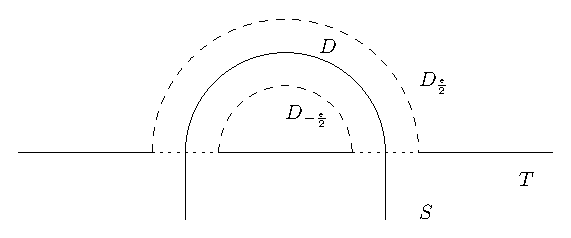
\includegraphics[width=0.54\textwidth]{surgery}
                \caption{Ausschneiden einer Umgebung von $S\cap T$ und Ankleben zweier Scheiben, sodass die Homologieklasse erhalten bleibt}
                \label{fig:surgery}
            \end{wrapfigure}
            Angenomme es existiert so ein Nullbordismus $D\subset S$ einer solchen Komponente $\partial D \subset S \cap T$. Weiter sei dieser auf dem Inneren disjunkt von $T$, da ein nichttrivialer Schnitt mit $T$ einen weiteren Kreis aus $S\cap T$ liefert, der den Nullbordismus einschränkt, sodass er weniger Komponenten im Schnitt mit $T$ berührt hat als der ursprüngliche (man bemerke das Transversalität genutzt wurde). So fahre man endlich oft fort, bis der Durchschnitt trivial ist beziehungsweise die berandende Scheibe, $T$ nur im Rand berührt.
            Nun lässt sich eine hinreichend kleine offene Tubenumgebung von $\partial D$ aus $T$ entfernen. Diese kann wie folgt gewählt werden: sei $\nu(S) \to M$ eine Tubenumgebung von $S$ die sich aufgrund der Zweiseitigkeit wie folgt wählen lässt: $\alpha: S \times (-\epsilon,\epsilon) \to M$, sodass $\im\alpha|_{S\times (-\frac 12\epsilon,\frac 12 \epsilon)} \cap T$ eine Tubenumgebung von $S\cap T \subset T$ ist. Dann lässt sich diese Tubenumgebung bei $\partial D$ aus $T$ entfernen und mittels der Zweiseitigkeit um $D$, findet man zwei Kopien $D_{\frac \epsilon 2}, D_{-\frac \epsilon 2}$, sowie Anklebevorschriften, mit denen diese Scheiben an die beiden durch Ausschneiden entstandenden Kreis-Randkomponenten kleben kann, vergleiche Abbildung~\ref{fig:surgery}. Als Resultat ergeben sich Flächen $S,T'$, deren Durchschnitt um eine Komponente reduziert wurde und offensichtlich $[T]=[T']$ gilt. \todo{kein Weg aus dem Durchschnitt ist rel Endpunkt homotop zu einem Rand}

            Von nun an seien $S,T$ transversale Flächen, deren Durchschnitt den obigen Anforderungen genügt. Ziel ist es nun, den Zykel, der die Vereinigung repräsentiert, als eingebettete Fläche zu repräsentieren. Beachtet man die Orientierungen, so kann man an jeder Komponente des Durchschnitts die Vereinigung aufschneiden (die lokal aussieht wie die Gerade an der sich zwei orientierte Ebenen im $\RR^3$ schneiden), und entlang der Orientierungen in nur einer Möglichkeit wieder verkleben, so dass man eine Mannigfaltigkeit erhält (dies funktioniert offensichtlich an den Durchschnittkomponenten mit Rand, aber auch den den geschlossenen Komponenten, da die Orientierungen auf $S$ und $T$ global gewählt sind). Natürlich können mit entsprechenden Umgebungen, alle diese Klebe- und Schneideprozesse glatt durchgeführt werden. Nun erhält man eine glatte, orientierte Fläche $U$, die (nach gegebenfalls leichter Modifikation) auch eigentlich eingebettet ist. Nun muss dieses Ergebnis und die Auswirkungen der Konstruktionen auf die Flächen diskutiert werden. Die "`uneinschränkenden"' Konstruktionen zu Beginn, können natürlich die Euler Charakteristik verändern, jedoch resultieren daraus weiterhin Thurston-Norm minimierende Flächen\footnote{Dies geschieht zum Beipsiel durch die Entstehung von Sphären. Wichtig ist nur dass solche Komponenten nicht beim Verkleben der beiden Flächen entstehen. Genau deswegen wurde diese Annahme getroffen.}. Zwei \emph{solche} Flächen gegeben, erbt die letztere Konstruktion, die aus $S\cup T$ eine homologe Fläche $U$ macht, die Summe der Eulercharakteristika:
            \begin{eqnarray*}
                \chi(U) = \chi(S) + \chi(T) &\implies& \chi_-(U)=\chi_-(S) + \chi_-(T) 
            \end{eqnarray*}
            wobei die Implikation gilt, da bei der Konstruktion von $U$ keine Komponenten mit positiver Eulercharakterstik entstehen, unter den an $S$ und $T$ gestellten Annahmen. Dies liefert nun die Subbadditivität der Thurston-Norm auf den Homologieklassen.
        \qed
        \vspace{6pt}

        Häufig stellt man Annahmen an die 3-Mannigfaltikeit, die es verbieten, dass Homologieklassen von Sphären oder Tori repräsentiert werden können. In dem Fall würde dann sogar $||\phi||_T=0 \Leftrightarrow \phi=0$ gelten. Dies alles motiviert natürlich, diese Norm zu einer Vektorraumnorm auf $H^1(M;\QQ)$ oder $H^1(M;\RR)$ fortzusetzen. 
        \begin{bem}[Fortsetzung von $||\cdot||_T$]
        \label{rem:extendingthurston}
            Will man $||\cdot||_T: H^1(M;\ZZ) \to \RR$ fortsetzen, so hilft die in Lemma~\ref{lem:norm} gezeigte Skalarmultiplikativität. Da $H^1(M;\ZZ)$ als $\ZZ$-Modul frei mit Rang $n$ ist, liefert die Einbettung $\ZZ^n \into \QQ^n$ zusammen mit der Linearität der Thurston-Norm eine lineare Fortsetzung auf den Strahlen (1-dimensionale Untervektorräume), die von Gitterpunkten erzeugt werden. Da aber für jedes $q \in \QQ^n$, bereits $aq \in \ZZ^n$ gilt (für großes $a\in \ZZ$), liefert dies bereits eine Fortsetzung auf $H^1(M;\QQ)$. Nun ist aber diese Fortsetzung mit Lemma~\ref{lem:norm} eine Halbnorm, insbesondere eine konvexe Funktion, also auf jedem Kompaktum Lipschitz-stetig und somit auf jedem Kompaktum $K\cap \QQ^n, K\subset \RR^n$ in eindeutiger Weise stetig auf $K$ fortsetzbar --- es folgt die Existenz von $||\cdot||_T:H^1(M;\RR) \to \RR$.
        \end{bem}
        Nun stehen die Definitionen der Invarianten bereit, die auf den folgenden Seiten untersucht werden sollen.

%!TEX root = main.tex


\section{Vorbereitungen der benötigten Theorien}
\label{sec:vorbereitungen}

\subsection{Über noethersche Moduln und Gruppenringe}
\label{sec:noetherianprinciples}
Im Folgenden sei $R$ stets ein kommutativer Ring mit $1\neq 0$.

Sei $M$ ein $R$-Modul. Dann ist $M$ noethersch, falls jeder Untermodul endlich erzeugt ist, insbesondere $M$ selbst. Ein Ring ist noethersch wenn er es als Modul über sich selbst ist. 

Da für jeden $R$-Modulhomomorphismus $M\to N$ das Bild der Erzeuger von $M$ das Bild des Homomorphismus erzeugt, gilt folgende Proposition:
\begin{prop}
	Sei $M \onto N$ ein $R$-Modulepimorphismus. Dann impliziert die endliche Erzeugbarkeit von $M$ die von $N$. \qed
\end{prop}
\begin{cor}
	Quotienten von endlich erzeugten Moduln sind endlich erzeugt. \qed
\end{cor}
\begin{cor}
\label{cor:noethchaincomplex}
	Sei $C_\bullet$ ein Kettenkomplex von noetherschen $R$-Moduln. Dann ist die Homologie endlich erzeugt über $R$.\qed
\end{cor}

\begin{lem}
\label{lem:epimorphismusnoethersch}
	Ein Epimorphismus von einem noetherschen $R$-Modul $M$ in einen weiteren $R$-Modul $L$ impliziert, das $L$ noethersch ist.
\end{lem}
\begin{proof}
	Jeder Untermodul aus $L$ besitzt ein endliches Erzeugendensystem als Bild endlich vieler Erzeuger des zurückgezogenen Untermoduls.
\end{proof}
\begin{lem}
\label{lem:exaktnoethersch}
	Sei $\seq LMN$ eine kurze exakte Sequenz von $R$-Moduln. Dann ist $M$ noethersch genau dann wenn $L$ und $N$ noethersch sind.
\end{lem}
\begin{proof}
	Sei $M$ noethersch, so ist es mit Lemma~\ref{lem:epimorphismusnoethersch} auch $N$. Weiter ist $L$ isomorph zum noetherschen Untermodul $\ker(M\to N)$. Umgekehrt erhalten wir für jeden Untermodul $M'\subset M$ eine kurze exakte Sequenz von Untermoduln mit den entsprechenden Einschränkungen $\seq {L'}{M'}{N'}$ wobei $L'$ und $N'$ als $R$-Untermoduln endlich erzeugt, somit auch $M'$.
\end{proof}

Sei im Folgenden $M$ noethersch. Dies ist zum Beispiel bei folgender Situation gegeben:
\begin{cor}
	Sei $R$ noethersch und $M$ ein endlich erzeugter $R$-Modul. Dann ist $M$ noethersch.
\end{cor}
\begin{proof}
	Mit Lemma~\ref{lem:exaktnoethersch} ist die direkte Summe $R^n$ noethersch und mit Lemma~\ref{lem:epimorphismusnoethersch} ist es $M$.
\end{proof}
\begin{lem}
	$M$ ist über $R$ endlich präsentiert. 
\end{lem}
\begin{proof}
	$M$ ist als größter Untermodul endlich erzeugt über $R$ also existiert folgende exakte Sequenz:
	\[
		R^n \to M \to 0.
	\]
	Da $R^n$ aber noethersch ist und Kerne von Homomorphismen Untermoduln sind, kann die Sequenz auf der linken Seite folgendermaßen ergänzt werden:
	\[
		R^m \to R^n \to M \to 0.
	\]
\end{proof}

 Für eine solche freie Auflösung von $M$, die also für noethersche Moduln immer existiert, sind alle Relationen durch $\ker(R^n\to M)$ gegeben. Deswegen nennt man eine darstellende Matrix zur Abbildung $f$ aus $R^m \stackrel f \to R^n \onto M$ auch Präsentationsmatrix. Verschiedene Präsentationsmatrizen unterscheiden sich nur durch die folgenden Operationen, siehe etwa~\cite[Theorem~6.1]{LickorishW.B.Raymond.1997}:
	(1) Vertauschen von Zeilen oder Spalten (2) Hinzufügen von Einheitsblöcken (als Blockmatrix oder direkter Summe mit der Identität) (3) Hinzufügen von Nullspalten und (4) Addieren eines Vielfachen einer Spalte oder Zeile auf eine jeweils andere. Zusammen mit grundlegenden Eigenschaften der Determinante liefert das die Wohldefiniertheit der folgenden Definition:
	\begin{defn}
	Es sei $R^m \to R^n \onto M$ eine endliche Präsentation des $R$-Moduls $M$ mit einer Präsentationsmatrix $X \in R^{n \times m}$. Definiere das $i$-te Elementarideal $E_i(M) \subset R$, als das von den Determinanten der $(n-i)\times (n-i)$-Minoren von $X$ erzeugte Ideal.
    	\end{defn}

        Da sich jede Determinante als Linearkombination von den Determinanten der Minoren schreiben lässt, ergibt sich eine Inklusionsbeziehung der Elementarideale. Für $n-i\leq 0$ und $n-i > \min(m,n)$ definiert man die Elementarideale gemäß der folgenden aufsteigenden Kette (da ohne Einschränkung $m>n$):
        \[
             0=E_{-1}(A)\subset E_0(A) \subset \cdots \subset E_n(A) = R
         \] 

        \begin{bsp}
        \label{bsp:hauptidealelementarteiler}
            Ist $R$ ein Hauptidealring, so sind die Elementarideale durch den Elementarteilersatz vollständig charakterisiert.
        \end{bsp}
        \begin{bem}
        	Das letzte Beispiel verwendet die Ergiebigkeit der Theorie der endlich erzeugten Moduln über Hauptidealringen. Die Elementarideale definieren nach den obigen Überlegungen Invarianten für endlich erzeugte Moduln über noetherschen Ringen. Dies ist durch eine Art Nachahmung der ersten Schritte des Elementarteilersatzes motiviert, die nur die endliche Präsentation der Moduln verwendet.
        \end{bem}

    Nun wird es später häufig nötig, Berechnungen über dem Gruppenring durchzuführen. Dafür wollen wir uns nun der Definition des Gruppenrings zuwenden und einige --- für Berechnungen essenzielle -- grundlegenden Eigenschaften des ganzzahligen Gruppenrings über einer frei abelschen Gruppe feststellen.

     \begin{defn}[Gruppenring]
    		Sei $G$ eine endlich erzeugte Gruppe. Dann ist der \textit{Gruppenring} definiert als die Menge aller endlichen formalen Summen:
    		\[
    			R[G] = \sum_{g \in G} a_g g, a_g \in \ZZ, g \in G
    		\]
            die durch komponentenweise Addition eine abelsche Gruppe wird und durch die Gruppenverknüpfung und die multiplikative Struktur von $R$ ein Ring mit Eins wird. Die Elemente $g \in G \subset R[G]$ werden als die Gruppenelemente in dem Gruppenring bezeichnet.
    	\end{defn}
    	Wir werden uns ausschließlich mit ganzzahligen oder rationalen Gruppenringen befassen, also mit $R \in \{ \ZZ,\QQ\}$.
    	\begin{bem}
    	\label{bem:gruppenwirkungmodul}
    		Sei also $M$ ein $R$-Modul mit einer Gruppenwirkung von $G$. Dann lässt sich $M$ als $R[G]$-Modul auffassen. Insbesondere werden wir also abelsche Gruppen und $\QQ$-Vektorräume über dem ganzzahligen bzw.\ rationalen Gruppenring betrachten.
    	\end{bem}
        \begin{bem}
            Da der Gruppenring die multiplikative Struktur von der Gruppenverknüpfung erbt, ist $\ZZ [G]$ im Allgemeinen nicht unbedingt kommutativ. Mit diesem Problem, das durch nicht-abelsche Gruppen $G$ entsteht, werden wir uns später beschäftigen müssen.
        \end{bem}
\begin{bsp}
        Falls $G$ eine unendlich zyklische Gruppe mit Erzeuger $t$ ist, lässt sich der Gruppenring über $F$ als $\ZZ[F] = \ZZ[t^{\pm 1}]$, also als Ring der formalen Laurentpolynome in der Variablen $t$ auffassen. 
\end{bsp}
Tatsächlich gilt dies sogar etwas allgemeiner. Dies wollen wir zeigen um Eigenschaften für den ganzzahligen Gruppenring zu entwickeln, die wir aus dem multivariablen Laurentring ableiten. Für diesen gilt nämlich:
\begin{prop}
	Der Laurentring $\ZZ[X_1^{\pm 1},\cdots,X_{n}^{\pm 1}] $ ist noethersch.
\end{prop}
\begin{proof}
	Nach dem Hilbertschen Basissatz ist der Polynomring über $\ZZ$ in endlich vielen Variablen noethersch. Ebenso ist die Lokalisierung eines noetherschen Ringes noethersch, da jedes Ideal in der Lokalisierung Bild eines endlich erzeugten Ideals ist. 
\end{proof}

Da der Laurentring mit $\ZZ$-Koeffizienten kein Hauptidealring ist, ist die vorhergehende Proposition so bedeutend. Die folgende Proposition wird zeigen, dass $\ZZ[F]$ für einen freien $\ZZ$-Modul $F$ auch kein Hauptidealring ist. Man sollte sich also um eine möglichst vollständige Liste guter Eigenschaften von $\ZZ[F]$ bemühen.

\begin{prop}
\label{prop:gruppenringnoethersch}
	Sei $F$ eine freie abelsche Gruppe, also $F\cong \ZZ^b$. Dann existiert ein Isomorphismus zwischen $\ZZ[F]$ und $\ZZ[X_1^{\pm 1},\cdots,X_{b}^{\pm 1}]$. Insbesondere ist $\ZZ[F]$ faktoriell und noethersch.
\end{prop}
\begin{proof}
	Unter Ausnutzung der universellen Eigenschaft des Polynomrings und der Lokalisierung definiert man folgende Abbildung:
	\begin{align*}
			\ZZ[X_1^{\pm 1},\cdots,X_{n}^{\pm 1}] & \to  \ZZ[F]\\
			X_i &\mapsto  f_i
	\end{align*}
	Wenn $f_i$ eine Basis von $F$ darstellt, so erhält man offensichtlich einen Isomorphismus.
\end{proof}

\begin{bem}
\label{bem:einheitengruppenring}
	Unter dieser Identifikation ergibt sich, dass die Einheiten $\ZZ[F]^\times$ genau die Produkte der Gruppenelemente mit den Einheiten von $\ZZ$ sind also $\pm F \subset \ZZ[F]$.
\end{bem}

Der Quotientenkörper von $\ZZ$ besitzt natürlich mehr Einheiten, deswegen ergibt sich für den Laurentring über $\QQ$ die Eigenschaft eines Hauptidealrings.
\begin{lem}
\label{lem:QThauptidealring}
	$\laurent\QQ t$ ist ein Hauptidealring.
\end{lem}
Natürlich könnte man $\QQ$ für dieses Lemma durch jeden beliebigen Körper $\KK$ ersetzen. 
%Allerdings entfällt durch Tensorieren mit einem endlichen Körper nicht jegliche Torsion, entsprechend birgt das mögliche Probleme bei Anwendung des universellen Koeffiziententheorems, da der $\Tor$ Anteil nicht zwangsweise verschwindet und somit gilt Proposition~\ref{prop:tensoring} nicht mehr.
\begin{proof}
	Da $\QQ$ ein Körper ist, ist $\QQ[t]$ ein Hauptidealring. Der Beweis läuft durch Betrachtung der kanonische Lokalisierungsabbildung:
	\[
		\alpha : \QQ[t] \to \laurent \QQ t
	\]
	Die Ideale in der Lokalisierung sind genau die erweiterten Ideale aus dem ursprünglichen Ring, wegen der Erhaltung durch $\laurent \QQ t \supset I=\alpha_*(\alpha^*(I))$, wobei $\alpha^* = \alpha^{-1}$ die Kontraktion eines Ideals bezeichnet und $\alpha_*(I) = \laurent \QQ t \cdot \alpha(I)$ die Erweiterung eines Ideals. Da aber jedes Element in $\laurent \QQ t$ durch Multiplizieren mit der Einheit $t^N$ im Erzeugnis eines Polynoms liegt, wird ein Erzeuger aus dem Hauptideal $\alpha^*(I)$ auf einen Haupterzeuger in $I$ abgebildet. 
\end{proof}
 Nun ist allgemeiner die Eigenschaft für einen Ring ein Hauptidealring zu sein, abgeschlossen unter Lokalisierungen. Der Beweis geht analog: Das Multiplizieren mit der Einheit $t^N$ führt einfach zu Multiplikation mit Elementen aus der multiplikativen Menge an der lokalisiert wurde --- den neuen Einheiten aus dem lokalisierten Ring.




	% Nach dem Hilbertschen Basissatz ist der Polynomring über $\ZZ$ in endlich vielen Variablen noethersch. Ebenso ist die Lokalisierung eines noetherschen Ringes noethersch, da jedes Ideal in der Lokalisierung Bild eines endlich erzeugten Ideals ist. 
	% Also genügt es eine Surjektion von einem solchen in den Gruppenring zu finden, denn ein surjektiver Ringhomomorhpismus ordnet jedem Ideal im überlagerten Ring ein endlich erzeugtes Ideal im ursprünglichen Ring zu und somit auch ein endliches Erzeugendensystem. Aber ein solcher Epimorphismus von einem --- nach den obigen Überlegungen --- noetherschen Ring ist gegeben durch Ausnutzen der universellen Eigenschaft des Polynomrings und der Lokalisierung:
	% \begin{align*}
	% 		\ZZ[X_1^{\pm 1},\cdots,X_{n}^{\pm 1}] & \to  \ZZ[F]\\
	% 		X_i &\mapsto  f_i
	% \end{align*}


\subsection{Poincaré und Lefschetz Dualität --- eine differentialtopologische Betrachtung}
\label{sec:poinc}

	Die Definition der Thurston-Norm in Kapitel~\ref{sec:thurstondef} wird uns eine Invariante auf $H^1(M;\ZZ)$ einer glatten Mannigfaltigkeit $M^m$ liefern, die durch Poincaré bzw.\ Lefschetz Dualität aus einer Invarianten auf $H_{m-1}(M,\partial M;\ZZ)$ hervorgeht. Und tatsächlich werden die folgenden Seiten teilweise in ein wildes Hin- und Herspringen zwischen Homologie und Kohomologie ausarten. Aus diesem Grund sollen hier noch einmal wichtige Grundlagen und Berechnungsmöglichkeiten, die später verwendet werden, erklärt werden.

	Zunächst widmen wir uns einigen Konventionen und Identifikationen.
	        \begin{bem}[Homomorphismen der Abelianisierung]
            \label{bem:fundhomologie}
            Es werden stillschweigend natürliche Identifikationen $H^1(M;\ZZ) \cong \Hom(H_1(M);\ZZ) \cong \Hom(\pi_1(M);\ZZ)$ verwendet. Die erste natürliche Identifikation liefert das universelle Koeffiziententheorem. Auch wenn die erhaltende Sequenz im Allgemeinen nicht natürlich zerfällt, so ist dies im Fall der ersten Kohomologie offensichtlich. Die zweite folgt, da ein Homomorphismus $\phi: H_1(M) \to \ZZ$ gleichbedeutend mit einem Homomorphismus $\hat\phi : \pi_1(M) \to \ZZ$ ist. Dies sieht man wie folgt ein: das Hurewicz Theorem besagt, dass die natürliche Abbildung $\pi_1(M) \to H_1(M)$, die durch Auffassen von Schleifen als singuläre 1-Zykel entsteht, die Abelianisierungsabbildung ist. Diese besitzt die universelle Eigenschaft der Quotientenabbildung zu dem Normalteiler $[\pi_1(M),\pi_1(M)]$. Da $\ZZ$ abelsch ist, folgt $[\pi_1(M),\pi_1(M)] \subset \ker \hat \phi$. Also faktorisiert $\hat \phi$ über eine eindeutige Abbildung $H_1(M) \to \ZZ$. Mit anderen Worten: Das folgende Diagramm kommutiert:
            \[
                \begin{xy}
                    \xymatrix{\pi_1(M)\ar[r]^{\hat \phi} \ar[d] & \ZZ \\
                                H_1(M)\ar[ru]_\phi}
                \end{xy}
            \]
            Dies liefert die eins-zu-eins Beziehung, da $\phi$ nach dem Diagramm offensichtlich ein eindeutiges Element in $\Hom(\pi_1(M);\ZZ)$ definiert. \\ \par
            \noindent\textbf{Konvention.} \emph{In dieser Arbeit bezeichne der Kern einer Klasse $\phi \in H^1(M;\ZZ)$ durchweg den Kern der mit $\phi$ identifizierten Abbildung auf der Fundamentalgruppe.}\\ \par
        \end{bem}
	\begin{bem}[Weitere Identifikationen]
	\label{bem:identifications}
	Sei $N$ eine glatte orientierte $n$-dimensionale Mannigfaltigkeit (mit CW-Struktur).
		Bekanntlicherweise gilt:
		\[
					H_{n-1}(N,\partial N;\ZZ)\cong H^1(N;\ZZ) \cong \Hom(H_1(N),\ZZ) \cong \Hom(\pi_1(N),\ZZ) \cong  [N,S^1]
		\]		
		wobei der
		\begin{enumerate}
			\item -te Isomorphismus bei $\partial N= \emptyset$ nach Poincaré und sonst Lefschetz Dualität,
			\item -te Isomorphismus gilt, da das universelle Koeffiziententheorem eine exakte Sequenz liefert in der diese beiden Terme auftauchen und weiter nur $\Ext(H_0(N),\ZZ) = 0$,
			\item -te Isomorphismus gilt, da nach Hurewicz die Abbildung $\pi_1(N)\to H_1(N)$ die Abelianisierung ist (siehe Bemerkung~\ref{bem:fundhomologie}),
			\item -te Isomorphismus gilt, indem man zeigt, dass jede Abbildung auf dem 1-Skelett $X^1 \subset N \to S^1$ auf $N$ fortgesetzt werden kann. Da das 1-Skelett die Fundamentalgruppe (oder Homologie) erzeugt, also die Inklusion eine surjektive Abbildung $i_*:\pi_1(X^1)\onto\pi_1(N)$ induziert, lässt sich auf diese Weise jeder Homomorphismus $\pi_1(N)\to \ZZ$ auf den Erzeugern aus dem 1-Skelett (genauer möchte man, dass diese Abbildung auf einem maximalen Baum konstant ist) definieren und fortsetzen. 
		\end{enumerate}


	\end{bem}
	\begin{bem}[Untermannigfaltigkeiten als Homologieklassen]
	\label{bem:untermannigfaltigkeitenalshomologie}
		Es sei $S^s$ eine $s$-dimensionale orientierte kompakte Mannigfaltigkeit. Die Orientierung liefert eine eindeutige Fundamentalklasse $[S] \in H_s(S)$ falls $S$ geschlossen ist und sonst $[S,\partial S] \in H_s(S,\partial S)$. Es sei $h:(S^s,\partial S) \into (N^n,\partial N)$ eine Einbettung. Dann definiert diese Einbettung eine Homologieklasse in $H_s(N,\partial N)$ als das Bild der eindeutigen Fundamentalklasse von $S$ unter der induzierten Abbildung $H_s(h)$. Für eine orientierbare kompakte Untermannigfaltigkeit $(S,\partial S) \subset (N,\partial N)$ liefert die Inklusion eine Einbettung und für eine gewählte Orientierung erhält man also eine Homologieklasse $[S]$ oder $[S,\partial S]$ in $H_s(N,\partial N)$.
	\end{bem}
	\begin{thm}
		Sei $f:N^n\to K^m$ eine stetige Abbildung glatter Mannigfaltigkeiten. Dann lässt sich $f$ beliebig nah durch glatte Abbildungen approximieren (wie die Güte der Approximation genau gemessen wird ist hier von keiner Bedeutung), welche homotop zu $f$ sind.
	\end{thm}
	\begin{thm}[Sard und Satz vom regulären Wert]
		Sei $f:N^n \to K^m$ eine glatte Abbildung. Dann liegen die regulären Werte von $f$ dicht in $K$. Das Urbild eines regulären Wertes ist eine abgeschlossene glatte orientierte eigentlich eingebettete Untermannigfaltigkeit in $K$ der Kodimension $m$. Ein regulärer Wert ist ein Punkt aus $K$, bei dessen Urbild $f$ an jedem Punkt einen Epimorphismus auf den Tangentialräumen definiert. 
	\end{thm}
	\begin{thm}[Thom]
	\label{thm:thom}
		Sei $f:N \to S^1$ eine glatte Abbildung. Jedes Urbild eines regulären Wertes definiert nach obigem Theorem und der Bemerkung~\ref{bem:untermannigfaltigkeitenalshomologie} ein Element in $H_{n-1}(N,\partial N;\ZZ)$. Diese ist Poincaré beziehungsweise Lefschetz dual zu $[f]\in H^1(N;\ZZ)$.
	\end{thm}
	Alle diese Aussagen sind bekannte elementare Aussagen der Differentialtopologie und können etwa in \cite{Kreck.2010} oder mit elementaren Methoden in \cite{Hirsch.1991} (bis auf \ref{thm:thom}) nachgelesen werden. 

	Das Zusammentragen aller Ergebnisse bedeutet also: Jeder Homomorphismus $\phi \in H^1(N;\ZZ)$ definiert ein eindeutiges Element in $[N,S^1]$. Umgekehrt liefert jede Abbildung $N\to S^1$ einen induzierten Homomorphismus der Homologiegruppen. Die Differentialtopologie liefert nun die restlichen Schritte. Jede Homotopieklasse aus $[N,S^1]$ enthält einen glatten Repräsentanten. Für diesen existiert ein regulärer Wert in $S^1$. Jedes Urbild eines solchen regulären Wertes ist dann eine 1-kodimensionale orientierte Mannigfaltigkeit (mit Rand, wenn überhaupt, im Rand von $N$ eigentlich eingebettet), welche als Homologieklasse dual zu $\phi$ ist.

	\subsection{Konstruktionen}
	Als explizite Anwendung des letzten Kapitels leiten wir in diesem Kapitel Konstruktionen her, die gewisse Informationen von 1-kodimensionalen Mannigfaltigkeiten beinhalten.
	\begin{lem}
		Wenn $M$ eine glatte orientierte $n$-Mannigfaltigkeit ist und $N\subset M$ eine glatte $k$-dimensionale Untermannigfaltigkeit, dann korrespondieren die Orientierungen von $N$ bijektiv mit den Orientierungen von dem Normalenbündel $\nu (N;M)$ in $M$.
	\end{lem}
	\begin{proof}
		Das Tangentialbündel von $N$ kann als Untervektorraumbündel von $TM$ aufgefasst werden; es ist unabhängig von der Einbettung. Falls $N$ nicht orientierbar ist, so ist es auch $\nu(N;M)$ nicht und umgekehrt. Sei also $N$ orientierbar, dann gilt für alle $x \in N$, dass die Faser $TN_x\oplus \nu(N;M)_x = TM_x$ die Orientierung von $M$ trägt, also $m_1,\cdots,m_n$ eine repräsentierende Basis der eindeutigen Orientierung ist. Also liefert die Lineare Algebra aus einer Orientierung von $N$, definiert durch die Basis des Tangentialraumes $n_1,\cdots,n_k$ eine eindeutige Orientierung von $\nu(N;M)_x$, repräsentiert durch die Basis $\nu_1,\cdots,\nu_{n-k}$, sodass die folgenden Orientierungen übereinstimmen: $[m_1,\cdots,m_n] = [n_1,\cdots,n_k,\nu_1,\cdots,\nu_{n-k}] $
	\end{proof}

	\begin{defn}
		Eine Untermannigfaltigkeit $N\subset M$ der Kodimension 1 heißt zweiseitig, falls eine glatte Einbettung $N \times (-\epsilon,\epsilon) \into M$ existiert, die auf $N \times \{0\} $ mit der Inklusion von $N$ übereinstimmt. Eine solche Einbettung heißt auch zweiseitiger Kragen.
	\end{defn}
	\begin{bem}
	\label{bem:zweiseitigkeit}
		Offensichtlich ist die Zweiseitigkeit einer 1-kodimensionalen Untermannigfaltigkeit gleichbedeutend mit einer Orientierung, da $N \times (-\epsilon,\epsilon)$ diffeomorph zu $\nu(N;M)$ ist. Falls wir im Folgenden von einer orientierten 1-kodimensionale Mannigfaltigkeit $N$ in einer orientierten Mannigfaltigkeit $M$ reden, so soll ihr zweiseitiger Kragen stets kompatibel gewählt sein. Das bedeutet, dass Urbilder von Repräsentanten der induzierten Orientierung des Normalenbündels, in $N\times (0,\epsilon)$ liegen.
	\end{bem}

Da wir im Folgenden nur 3-Mannigfaltigkeiten betrachten, so gestatten wir jetzt schon die Bequemlichkeit uns auf solche zu reduzieren. Die 1-kodimensionalen Untermannigfaltigkeiten sind also diffeomorph zu Flächen.

\label{sec:constr}
Zu einer gegebenen Homologieklasse $  \phi \in H^1(M;\ZZ)$ finden wir nach Kapitel~\ref{sec:poinc}, sowohl den eindeutigen Homomorphismus $\phi:\pi_1(M) \to \ZZ$ als auch eine glatte Abbildung $f:M \to S^1$ die $\phi$ induziert. Außerdem finden wir mit Kapitel~\ref{sec:poinc} eine zu $ \phi$ duale orientierte Untermannigfaltigkeit $S$ als Urbild eines Punktes unter $f$. Mit den folgenden Konstruktionen soll bewiesen werden, dass jede duale orientierte eingebettete Fläche $(S,\partial S) \subset (M,\partial M)$ als Urbild eines regulären Wertes darstellbar ist. Weiter wollen wir häufig die zu $\ker \phi$ gehörige Überlagerung betrachten. Wir werden ein Verfahren entwickeln, in welchem wir durch Aufschneiden und Verkleben an $S$ diese Überlagerung erhalten. Genauer wollen wir zeigen: Sowohl durch Aufschneiden an $S$ als auch durch Zurückziehen der universellen Überlagerung von $S^1$ entlang $f$ erhalten wir die Überlagerung zu dem Normalteiler $\ker\phi$ der Fundamentalgruppe.

\begin{constr}[Aufschneiden an einer Fläche]
	\label{constr:cut}
	Aus der Überlagerungstheorie ist bekannt, dass zu jeder normalen Untergruppe der Fundamentalgruppe eines hinreichend gut zusammenhängendem Hausdorffraumes (insbesondere Mannigfaltigkeiten), auch eine normale zusammenhängende Überlagerung existiert, die bis auf Überlagerungsisomorphie eindeutig ist, siehe~\cite[Chapter~1.3]{Hatcher.2002}. Nun definiert aber ein Element $\phi\in H^1(M,\ZZ)$ nach obigen Überlegungen den Normalteiler $\ker\phi\subset \pi_1(M)$. In diesem Sinne nennen wir die Überlagerung zu $\phi$ fortan $M_\phi$.  Da jede duale Homologieklasse nach Kapitel~\ref{sec:poinc} eine Untermanigfaltigkeit als Repräsentanten besitzt, sei also $(S,\partial S) \subset (M,\partial M)$ eine eingebettete orientierte Fläche, deren Fundamentalklasse dual zu $\phi$ ist. Da diese Kodimension~$1$ und eine Orientierung hat, ist sie nach Bemerkung~\ref{bem:zweiseitigkeit} auch zweiseitig. Fixiere also einen zweiseitigen Kragen\footnote{Diese Zweiseitigkeit sei natürlich stets mit der Kompatibilität mit der induzierten Orientierung des Normalenbündels gewählt. Dies wurde auch in Bemerkung~\ref{bem:zweiseitigkeit} verlangt und bedeutet auch Kompatibilität mit der Orientierung.} $h:S\times (-\epsilon,\epsilon) \to M$. Das bedeutet, dass die 3-Mannigfaltigkeit an $S$ "`aufgeschnitten"' werden kann (siehe etwa~\cite[Kapitel~4.2]{Burde.2003}), wobei das Aufschneiden bedeutet, das Komplement der Fläche zu betrachten (das Resultat ist offensichtlich eine Mannigfaltigkeit, jedoch können Eigenschaften wie Kompaktheit oder Randbedingungen entfallen). Will man nun die durch Aufschneiden gewonnene Kopien $(M_i)_{i\in \ZZ}, M_i \cong M-S$ wieder verkleben, erweist sich die Zweiseitigkeit der Fläche als günstig, sogar notwendig (sonst würde nur \emph{eine} Kopie von $S$ als Rand entstehen). Der fixierte zweiseitige Kragen liefert nämlich durch $h(S,(-\epsilon,0))$ und $h(S,(0,\epsilon))$ offene Mengen $M_i^-$ und $M_i^+$ in den $M_i$. Durch die Diffeomorphismen $h_+: S\times (0,\epsilon) \to M_i^+$ und $h_-:S\times (-\epsilon,0) \to M_{i+1}^-$, können nun $M_i$ und $M_{i+1}$ jeweils entlang $M_i^+$ und $M_{i+1}^-$ an $S\times (-\epsilon,\epsilon)$ geklebt werden --- genauer: $h$ liefert eine Äquivalenzrelation auf der disjunkten Vereinigung 
	\[
		\cdots \sqcup M_{i-1} \sqcup (S \times (-\epsilon,\epsilon)) \sqcup M_i \sqcup  (S \times (-\epsilon,\epsilon)) \sqcup M_{i+1} \sqcup \cdots,
	\]
	sodass der Quotient eine unendlich zyklische Überlagerung mit der offensichtlichen Projektion bildet. Da entlang offener Mengen verklebt wird, also durch die "`Überlappungen"', ist es möglich den gewonnenen Quotienten mit einer differenzierbaren Struktur zu versehen, so dass die Inklusionen der $M_i$ glatte Einbettungen und somit Untermannigfaltigkeiten sind.

	Nun muss die resultierende Überlagerung keineswegs zusammenhängend sein. Wir werden später sehen, dass es aber hinreichend ist, wenn die Fläche $S$ zusammenhängend ist und nicht nullhomolog. Denn dann ist mit Corollar~\ref{cor:zshtrennendnullhomolog} das Komplement $M-S$ zusammenhängend. In den nächsten Betrachtungen sei die entstehende unendlich zyklische Überlagerung zusammenhängend.

	Als weiteren Vorteil dieser expliziten Konstruktion, sieht man explizit die Diffeomorphismen der unendlich zyklischen Decktransformationsgruppe mit Erzeuger $t$. Es entspricht $nt$ einer Translation aller $M_i$ um $n$. Es bleibt nur noch zu zeigen, dass diese Überlagerung auch \textit{die} zu $[S]$ gehörige Überlagerung ist, die in dem obigen Sinne dem dualen $\phi$ entspricht (da $S$ immer noch die gewählte Orientierung bzw.\ den gewählten zweiseitigen Kragen trägt). Dies sieht man zum Beispiel ein, indem man sich unter dem Isomorphismus $H^1(M;\ZZ)\cong [M,S^1]$ einen glatten Repräsentanten aussucht der $\phi$ induziert. Natürlich existiert so einer nach den Bemerkungen in~\ref{sec:poinc} immer, jedoch soll dieser für den gewünschten Nachweis explizit $S$ als orientiertes Urbild eines regulären Wertes ergeben. Dafür konstruiert man sich aus dem fixierten zweiseitigen Kragen eine Abbildung $f:M\to S^1$, die $S\times 0$ auf $p\in S^1$ abbildet, $M-(S \times (-\epsilon,\epsilon))$ konstant auf den antipodalen Punkt von $p$ abbildet und auf $S\times (-\epsilon,\epsilon)$ gemäß der Projektion auf den zweiten Faktor fortgesetzt wird. Bezüglich dieser glatt konstruierten Abbildung $f$ ist der Wert $p$ regulär und $f^{-1}p=S$ mit der richtigen Orientierung ausgestattet. Durch paralleles Aufschneiden von $M$ an $S$, und $S^1$ an $p$ (analog wie oben nur 2 Dimensionen tiefer) erhält man folgendes kommutatives Diagramm von zusammenhängenden Überlagerungen:
	\[
		\begin{xy}
			\xymatrix{M_\phi \ar[r] \ar[d] &\RR \ar[d]\\
						M \ar[r]& S^1}
		\end{xy}
	\]

	Dieses Diagramm ist ist aber nun ein Pullback-Diagramm von glatten Faserbündeln. Also ist die Diffeomorphieklasse von $M_\phi$ eindeutig. 
\end{constr}
Wir können festhalten:
\begin{cor}
\label{cor:verklvertr}
		Die unendlich zyklische Überlagerung, die durch Aufschneiden und Verkleben an einer zu $\phi$ dualen Fläche entsteht, entspricht der normalen Untergruppe $ \ker\phi$.
\end{cor}
\begin{cor}
\label{cor:preimage}
	Jede zu $\phi$ duale Fläche kann als orientiertes Urbild eines regulären Wertes einer glatten Abbildung $M\to S^1$ dargestellt werden, mit $H_1(M \to S^1)=\phi$.
\end{cor}
Mit einer zu $\phi$ dualen Fläche ist eine eigentlich eingebettete orientierte 1-kodimensionale Untermannigfaltigkeit gemeint, deren Einbettung die Fundamentalklasse auf eine zu $\phi$ duale Homologieklasse abbildet. Corollar~\ref{cor:preimage} gilt natürlich mit der obigen expliziten Angabe der glatten Abbildung für allgemeine $S$, auch solche deren Überlagerung durch Aufschneiden und Verkleben nicht zusammenhängend ist.

\begin{constr}[Graph einer orientierten 1-kodimensionalen Untermannigfaltigkeit]
	\label{constr:graph}
	Sei $S$ ein beliebiger zu $\phi \in H^1(M,\ZZ)$ dualer eigentlich eingebetteter, orientierter Repräsentant. Wir haben gesehen, dass mit obiger Konstruktion eine Abbildung $f:M\to S^1$ entsteht mit $f^{-1}p=S$. Diese Abbildung soll in dieser Konstruktion über einen Graphen faktorisiert werden.

	Bezeichne $S=S_1\sqcup \cdots \sqcup S_n$ und $M-S = M_1 \sqcup \cdots \sqcup M_m$ die Zusammenhangskomponenten von $S$ bzw. $M-S$. Man betrachte nun den gerichteten Graphen $G$, dessen Knoten bijektiv den Komponenten $M_i$ entsprechen und dessen Kanten aus den Komponenten $S_i$ mit ihrer Orientierung hervorgehen. Also ein Graph mit $m$ Knoten und $n$ Kanten, wobei eine Kante von einem Knoten zu einem anderen verläuft, wenn die korrespondierenden Komponenten $M_i, M_j$ durch das entsprechende Flächenstück von $S$ getrennt werden, sodass die Komponenten das zweiseitige Flächenstück an der negativen beziehungsweise positiven Seite berühren, je nachdem ob die Kante vom assoziierten Knoten aus oder eingeht.

	Mit genau diesen zweiseitigen Umgebungen der Flächenkomponenten ist es möglich, ähnlich wie oben eine Abbildung $M \to G$ zu definieren, welche die Assoziierungen respektiert. Dafür betrachte man den zweiseitigen Kragen auf den Komponenten von $S$:
	\[
		\sqcup (S_i \times (-\epsilon,\epsilon)) \stackrel = \longrightarrow S \times (-\epsilon,\epsilon) \into M
	\]
	Dann existiert analog zur obigen Konstruktion die Quotientenabbildung $q:M\to G$ auf den Graph, durch Kollabieren der $M_i\cap (M -S \times(-\epsilon,\epsilon))$ auf ihre Knoten und Projektion von $(-\epsilon,\epsilon)$ auf das Innere der Kanten des Graphen. Man betrachte außerdem $G \to S^1$ die Abbildung die jede Kante entsprechend ihrer Richtung, also orientierungserhaltend, einmal um die Sphäre $S^1 = I/\partial I$ abbildet, sodass die Knoten nach $[\partial I]$ abgebildet werden. Außerdem seien die Mittelpunkte der Kanten das Urbild von dem antipodalen Punkt von $[I/\partial I]$, etwa $p\in S^1$. Sei $f$ nach wie vor die Abbildung aus der letzten Konstruktion. Wir erhalten:
	
	\begin{align}
		\begin{xy}
				\xymatrix{M \ar[r] \ar@/^1pc/[rr]^f & G \ar[r] & S^1 }
			\end{xy}
		\label{eq:graphlift}
	\end{align}
	Da $M$ zusammenhängend ist, ist es auch $G$.
\end{constr}

\begin{cor}
	\label{cor:trennendeFlachen}
	Sei $S$ eine orientierte, eigentlich eingebettete Fläche und der dazugehörige Graph $G$ nach Konstruktion~\ref{constr:graph} habe einen Knoten $M_i$, mit nur ein- oder ausgehenden Kanten. Dann ist die Vereinigung $\hat S$ aller Komponenten von $S$ die $M_i$ berühren nullhomolog.
\end{cor}
\begin{proof}
	Im allgemeinen Fall betrachtet man den Graphen $F$ der aus Konstruktion~\ref{constr:graph} bezüglich $\hat S$ entsteht. Das Ergebnis dieser Konstruktion war es, dass die Komposition $M\to F \to S^1$ eine zu $[\hat S]$ duale Kohomologieklasse induziert (unter der Identifikationen aus Bemerkung~\ref{bem:fundhomologie}). Aber $F$ hat folgende Form:
\begin{center}
\begin{tikzpicture}[->,>=stealth',shorten >=1pt,auto,node distance=1.5cm,
  thick,main node/.style={circle,fill=black!1,draw}]

  \node[main node] (1) {};
  \node  (2) [below  of=1] {\huge{...}};
  \node[main node] (3) [below  of=2] {};
  \node (l2) [left of=2]{};
  \node (l) [left of=l2]{};
  \node (ll) [left of=l]{};
	\node (lll) [left of=ll] {$M$};
	\node (r2) [right of=2]{};
  \node (r) [right of=r2]{};
  \node (rr) [right of=r]{};
	\node [main node] (rrr) [right of=rr] {};
	\node (F) [right of=3] {$F$};
\node (S) [below of=rrr] {$S^1$};
  \path[every node/.style={font=\sffamily\small}]
    (1) 
        edge [bend angle=45,bend right] node[left] {$S_i$} (3)
        edge [bend angle=45,bend left]  node[right] {$S_j$} (3)
         edge [bend right] node[left] { } (3)
        edge [bend left]  node[right] { } (3)
     (ll) edge (l)
     (r) edge (rr)
    (rrr) 
    	edge[loop right, looseness=15, min distance=15mm] node { } (rrr);
\end{tikzpicture}
\end{center}

	  Jede Komposition $S^1 \to M \to F \to S^1$ hat somit Grad 0, aber da Homotopieklassen $[S^1,S^1]$ durch den Grad charakterisiert sind, ist somit $[\hat S]$ dual zu dem trivialen Homomorphismus $\pi_1(M) \to H_1(M) \to \ZZ$. Es gilt $[\hat S] = 0$.

	Ein elegantes Argument ergibt sich, wenn $M$ geschlossen ist. Dann faktorisiert die Inklusion der beteiligten Flächenkomponenten über einen orientierten Nullbordismus, nämlich $\overline{M_i}$ oder $M-M_i$. Mit der Funktorialität der Homologie, faktorisiert die Inklusion auf der zweiten Homologie dann über die induzierte Abbildung der Inklusion in den orientierten Nullbordismus, welche die Fundamentalklasse trivial auswertet\footnote{Das folgt aus der exakten Sequenz für das Paar $H_n(N^n, \partial N) \to H_{n-1}(\partial N) \stackrel i \to H_{n-1}(N^n)$, da der Randoperator die (relative) Fundamentalklasse auf die Fundamentalklasse des Randes abbildet und diese somit im Kern der Inklusion ist.}.
\end{proof}
\begin{cor}
\label{cor:zshtrennendnullhomolog}
	Sei $S$ eine zusammenhängende orientierte, eigentlich eingebettete Fläche, deren Komplement nicht zusammenhängend ist. Dann ist $[S]=0$.  
\end{cor}
\begin{proof}
	Mit der Zweiseitigkeit von $S$ folgt, dass der dazugehörige Graph aus Konstruktion~\ref{constr:graph} aus einer Kante und zwei verschiedenen Knoten besteht.
\end{proof}

Im Folgenden wollen wir häufig den Spezialfall betrachten, dass $\phi: H_1(M) \to \ZZ$ surjektiv ist. 
\begin{defn}
	Ein solches $\phi \in H^1(M;\ZZ)$ heißt primitiv.
\end{defn}

\subsection{Normen und Halbnormen auf freien $\ZZ$-Moduln und ihre Fortsetzungen}
    
    Ziel der folgenden Kapitel wird es sein, einer Diffeomorphieklasse von Mannigfaltigkeiten eine Halbnorm und somit eine Invariante zuzuordnen. Genauer gesagt werden es sogar mehrere Halbnormen sein. Die Halbnormen werden wir zunächst auf der ersten Kohomologie $H^1(M;\ZZ)$ definieren. Die erste Kohomologie eines kompakten topologischen Raumes ist stets torsionsfrei, denn es gilt: $H^1(M;\ZZ) \cong \Hom(H_1(M;\ZZ);\ZZ) \cong \Hom(H_1(M;\ZZ)/T;\ZZ) \cong \ZZ^n$, wobei $T$ der Torsionsanteil der abelschen Gruppe $H_1(M;\ZZ)$ ist. Es wurde $\Hom(T;\ZZ)=0$ und $H_1(M;\ZZ) \cong H_1(M;\ZZ)/T \oplus T$ verwendet.

    \begin{defn}
    	Eine ganzzahlige Halbnorm ist eine Abbildung $||\cdot||: \ZZ^n \to \ZZ$  die Skalarmultiplikativität und Subadditivität erfüllt. Also für alle $\lambda \in \ZZ$ und $v,w\in \ZZ^n$ soll $||\lambda v||=\vert\lambda\vert~||v||$ und die Dreiecksungleichung $||v+w||\le ||v||+||w||$ gelten.
    \end{defn}
    Es folgt natürlich aus der Skalarmultiplikativität, dass die $0$ trivial von der Halbnorm ausgewertet wird, da $||0|| = 0||0||$. Gilt auch die Umkehrung, also $||v||=0, v\in \ZZ^n \Rightarrow v=0$, so nennen wir $||\cdot ||$ eine ganzzahlige Norm. Analog seien rationale (Halb-)Normen und reelle (Halb-)Normen definiert. 
    \begin{lem}
    \label{lem:fortsetzungnorm}
    	Eine ganzzahlige Halbnorm lässt sich auf eine rationale Halbnorm fortsetzen. Eine ganzzahlige oder rationale Halbnorm lässt sich auf eine reelle Halbnorm fortsetzen. Das gleiche gilt für Normen.
    \end{lem}
    \begin{proof}
    	Möchte man $||\cdot||:  \ZZ^n \to \ZZ$ rational fortsetzen, so bemerkt man, dass die Einbettung $\ZZ^n \into \QQ^n$ die Norm bereits durch die geforderte Skalarmultiplikativität fortgesetzt wird. Sobald man einen Wert für einen Punkt auf einem 1-dimensionalen Unterraum hat, so hat man ihn bereits für den ganzen Unterraum. Jede Gerade durch den Ursprung in $\QQ^n$ schneidet einen und somit unendlich viele Gitterpunkte: Für jedes $q \in \QQ^n$ ist bereits $aq \in \ZZ^n$ für ein großes $a\in \ZZ$. Diese lineare Fortsetzung ist offensichtlich eine Halbnorm, sogar eine Norm, falls $||\cdot||$ es auf $\ZZ^n$ war.

    	Sei nun $||\cdot||: \QQ^n \to \QQ$ eine Halbnorm. Dann ist diese insbesondere eine konvexe Funktion, also auf jedem Kompaktum Lipschitz-stetig und somit auf jedem Kompaktum $K\cap \QQ^n, K\subset \RR^n$ in eindeutiger Weise stetig auf $K$ fortsetzbar --- es folgt die Existenz einer rellen Fortsetzung.
    \end{proof}



    \begin{bem}[Duale Vektorraumhalbnorm]
        Eine (Halb-)Norm auf einem Vektorraum, liefert stets eine (Halb-)Norm auf seinem Dualraum. Diese ist für einen Vektorraum $(V,|\cdot|)$ auf dem Dualraum $(V^*,||\cdot||)$ definiert durch:
        \[
             ||\alpha||= \sup_{\{v\in V, |v|=1\}} |\alpha v|
         \] 
         Entsprechend lässt sich eine Halbnorm auf $H^1(M;\RR)$ auf $H_1(M;\RR)$ durch den natürlichen Isomorphismus auf den Bidualraum definieren. Weiter lässt sich eine solche Halbnorm der ersten Kohomologie bei kompakten orientierbaren 3-Mannigfaltigkeiten mittels der Dualitätssätze auf $H_2(M,\partial M;\RR)$ übertragen, die wiederum durch Vektorraumdualität eine Halbnorm für $H^2(M,\partial M;\RR)$ liefert.
    \end{bem}


    \subsection{Die betrachteten Räume}
    	Nun noch eine letzte Generalvoraussetzung, die ab sofort verlangt wird:

       \emph{Im Folgenden sei $M$ stets eine kompakte, orientierbare, zusammenhängende $3$-dimen-sionale Mannigfaltigkeit. Falls diese einen Rand hat, sei er diffeomorph zu einer disjunkten Vereinigung von Tori.}

        Um die Hilfsmittel zu erweitern oder Extremfälle auszuschließen, arbeitet man häufig in der Kategorie der stückweise linearen (PL, \textit{piecewise linear}) oder der differenzierbaren Mannigfaltigkeiten. Sieht man sich beispielsweise topologische Knoten an, also stetige Einbettungen $S^1 \into S^3$, so stellt man fest, dass diese besonders ausgeartet aussehen können. Dies passiert jedoch nicht, falls es sich bei der Einbettung um eine PL oder eine differenzierbare Einbettung handelt. Ähnlich kann man in diesen Kategorien raumfüllende Kurven vermeiden. Allerdings stellte sich im Studium der $3$-Mannigfaltigkeiten heraus, dass die Situation sich erheblich von der in höheren Dimensionen unterscheidet. Beispielsweise ist nicht jede Gruppe als Fundamentalgruppe einer $3$-Mannigfaltigkeit realisierbar, eine Einschränkung liefert etwa Theorem~\ref{thm:keralexnorm}. Außerdem lässt sich die Tatsache ergiebig nutzen, dass in Dimension~$3$ keine Unterscheidung der topologischen, der PL und der differenzierbaren Kategorie nötig ist: Nach Moises Theorem (vgl.\,\cite{Moise.1952}) besitzt jede $3$-Mannigfaltigkeit sowohl eine eindeutige PL, als auch eine eindeutige differenzierbare Struktur. Das bedeutet, um Aussagen für $3$-Mannigfaltigkeiten zu zeigen, kann man sich (fast) beliebig in diesen Kategorien hin- und herbewegen, um das Resultat am Ende für alle zu erhalten. Um diese beiden Beispiele hervorzuheben, lässt sich bemerken, dass der $\RR^4$ überabzählbar viele unterschiedliche differenzierbare Strukturen besitzt und auch jede Gruppe realisierbar als Fundamentalgruppe einer $4$-Mannigfaltigkeit ist.

        Diese Arbeit wird sich jedoch konsistent in der $C^\infty$-Kategorie bewegen. Der vorherige Absatz dient also lediglich der Betonung, dass dies keine Einschränkung bedeutet. 
%!TEX root = main.tex

\section{Algebraische Alexander Invarianten}
\label{sec:algebra}
Tatsächlich könnte man diese Bachelorarbeit fast ausschließlich algebraisch verstehen --- wenigstens den Teil über die Alexander-Invarianten. Natürlich ist dieser Arbeit aus dem Bereich der Topologie, der Geschmack oder die Illusion gegeben, man arbeite mit direkten Eigenschaften der Räume. Bei der Thurston-Norm ist dies sicherlich noch eher gegeben, durch die Deftinition einar Funktion auf einem Vektorraum mittels geometrischer Eigenschaften der Mannigfaltigkeit. Jedoch handelt es sich bei den Alexander-Invarianten, insbesondere dem Alexander Polynom, lediglich um Invarianten einer endlich erzeugten Gruppe. Durch Anwendung dieser Invarianten auf die Fundamentalgruppe eines topologischen Raumes, erhält man also Invarianten von Räumen. Natürlich verliert das Alexander Polynom von 3-Mannigfaltigkeiten durch diese "`Faktorisierung"' nicht allzu viel an Reiz, da die Fundamentalgruppe eine recht starke Invariante von 3-Mannigfaltigkeiten darstellt, beispielsweise liefert sie durch einfache Anwendung von Hurewicz und Dualitätssätzen (Poincaré/Lefschetz, universelles Koeffiziententheorem) alle Homologiegruppen der 3-Mannigfaltigkeit und eine Klasse von 3-Mannigfaltigkeiten, die sogenannten `Haken-Mannigfaltigkeiten' sind durch ihre Fundamentalgruppe klassifiziert, der Beweis dazu stammt von Waldhausen~\cite{Waldhausen.1968}. Im Folgenden sollen nun die Alexander Invarianten von endlich erzeugten Gruppen definiert werden und Zusammenhänge verschiedener Definitionen erkannt werden.

Natürlich bergen algebraische Invarianten mit solchen Eigenschaften immer mehrere Vorzüge. Zum einen werden topologische Probleme in algebraische übersetzt, die dann mit algebraischen Methoden untersucht werden können. Scheint andererseits ein algebraisches Problem nur schwer lösbar, so ergibt sich die Möglichkeit einen topologischen Kontext zu finden, in dem sich die algebraische Ursprungssituation als Invariante ergibt, dessen Ergebnisse und Berechnungen sich aber vielleicht mit topologischen Eigenschaften des Raumes leichter handhaben lassen, siehe etwa Beispiel~\ref{ex:eilmaclane}.

Es soll zunächst eine analoge Definition zu den bekannten Alexander Invarianten aus Kapitel~\ref{sec:defs} gegeben werden. Anschließend wollen wir eine weitere Definition betrachten, die beispielsweise McMullen in \cite{MCMULLEN.2002} nutzt und ein Zusammenhang hergestellt werden --- warum diese Definitionen streng genommen nicht äquivalent sind und warum das kein Problem darstellt.

\subsection{Herleitung der algebraischen Idee}
    
Nun müssen wir uns mit der Problematik beschäftigen die eingangs bei der Definition des Gruppenrings erwähnt wurde, nämlich dass der entstehende Gruppenring von nicht-abelschen Gruppen nicht mehr kommutativ ist, man also beispielsweise zwischen Links- und Rechtsmoduln über dem Gruppenring unterscheiden muss.

Sei $G$ die Fundamentalgruppe von $M$ und $F$ eine freier abelsche Gruppe zusammen mit einem Epimorphismus $\alpha:G \to F$. Also faktorisiert $\alpha$ durch die maximale freie abelsche Quotientenabbildung $G \to G/[G,G] \to ab(G) \cong \ZZ^{b_1(G)}$ die als Komposition kanonischer Abbildungen kanonisch ist. Folglich ist der Rang von $F$ durch $b_1(G)$ nach oben beschränkt. Dann erhält man einen Gruppenisomorphismus $p'_*: H_1(\hat M) \to \ker\alpha/[\ker\alpha,\ker\alpha]$ der durch die Überlagerungsprojektion $\hat M = M_\alpha \to M$ zu $\alpha$ induziert wird. Ziel wäre es zu zeigen, dass diese Abbildung auch einen Isomorphismus von $\ZZ[F]$-Moduln liefert. Daraus würden natürlich gleiche Präsentationen folgen, die zu gleichen Elementaridealen führen und so fort. Hierfür benötigt man jedoch überhaupt eine $\ZZ[F]$-Modul Struktur auf dem Quotienten $G'/G''$ für $G'=\ker\alpha, G''=[G',G']$. Diese soll zunächst definiert werden:

Es seien $g_1,\cdots,g_m,m\leq b_1(G)$ Elemente die auf eine Basis von $F$ abgebildet werden. Diese definieren dann Automorphismen von $G'/G''$ durch 
\[
	\hat t_i(x) =  [g_i]  [x][ g_i^{-1}] = [ g_i x g_i^{-1}]
\]
Man prüft leicht, dass diese unabhängig der gewählten $g_i$ sind. Es sei für den Beweis bemerkt, dass die Kommutatoruntergruppe $G''\subset G'$ eine charakteristische Untergruppe ist. 
\begin{bem}
 	Das ist eine Form der expliziten Konstruktion des Falles, wenn man von einer induzierten Operation einer zerfällenden kurzen exakten Sequenz redet:
 	\[
 		\seq {G'/G''} {G/G''} {G/G'}
 	\]
 	Da $F= G/G'$ frei abelsch ist, zerfällt diese Sequenz und man erhält eine Abbildung $F \to \Aut(G'/G'')$ genauer gesagt, eine Gruppenwirkung auf $G'/G''$ durch Konjugation unter der Einbettung $G'/G''\into G/G''$ mit zurückgezogenen Elementen aus $F$. Dies ist wohldefiniert da das Bild von $G'/G''$ einem Kern entspricht, also Normalteiler ist. Offensichtlich stimmt diese Operation mit der obigen überein.
 \end{bem} 
 
 Mit $\alpha(g_i)=t_i$ als ein Element der Basis von $F$, ist die Gruppenwirkung von $F$ auf $H_1(\hat M)$, die durch die Decktransformationen $F$ induzierte $t_i\gamma = t_{i*}\gamma,t_i \in F , \gamma \in H_1(\hat M)$. Also ist nur zu zeigen, dass folgendes Diagramm kommutiert:
\[
	\begin{xy}
		\xymatrix{H_1(\hat M) \ar[d]_{t_i} \ar[r]^{p'_*} & G'/G'' \ar[d]^{\hat t_i}\\
		H_1(\hat M)  \ar[r]^{p'_*} & G'/G'' }
	\end{xy}
\]
und somit die Operationen verträglich sind. Davon überzeugt man sich, indem man die Wirkung von $t_i$ näher betrachtet: nach Hurewicz lässt sich ein Zykel aus $H^1(\hat M)$ als Schleife darstellen. Die Decktransformation $t_i$ bildet diese Schleife nun auf eine Schleife ab, die homolog ist zu der Konjugation mit einer zu einem Weg gelifteten Schleife $\tau_i, [\tau_i] \in \pi_1(M,p)$, welche die Decktransformation $t_i$ erzeugt. Aber wegen $\alpha([\tau_i])=t_i$ ist $\hat t_i$ auch nur Konjugation mit $\tau_i$.

Also lassen sich alle Definitionen der Alexander Invarianten analog zu Kapitel~\ref{sec:defs}, auf endlich erzeugten Gruppen definieren, wobei der Alexander Modul $G'/G''$ als Modul über $\ZZ [G/G']= \ZZ F$ aufgefasst wird. Fast! Die Definition der Elementarideale setzt noch voraus, dass dieser Modul endlich erzeugt ist. Wir hatten bisher nur gesehen, dass dies für Fundamentalgruppen von 3-Mannigfaltigkeiten stimmt, indem wir eine endliche CW-Struktur ausgenutzt haben. Dies wird am Ende des Kapitels festgestellt.

\begin{bem}
Es stellt sich sogar heraus, dass in den vielen Fällen auch die Thurston Norm, aus der Fundamentalgruppe berechnet werden kann, indem man getwistete Alexander Polynome verwendet --- die mit ähnlichen Methoden wie oben, allein aus der Fundamentalgruppe gewonnen werden können. Sie beinhalten meist noch mehr Daten als das gewöhnliche Alexander Polynom und es lässt sich mit dem induzierten Norm dieser Polynome, die Abschätzung aus Theorem~\ref{thm:haupttheorem} verallgemeinern. Diese Resultate wurden in mehreren Arbeiten von Friedl unter verschiedenen Zusammenarbeiten entwickelt, etwa in \cite{Friedl.2011,Friedl.2008,Friedl.2008b,Friedl.2007,Friedl.2006,Friedl.2008c}. Weiter nützen die getwisteten Alexander Polynome um bis zu einem gewissen Grade eine Umkehrung der Gleichheit aus Theorem~\ref{thm:haupttheorem} bei Faserungen zu ermöglichen, siehe~\cite{Friedl.2006,Friedl.2008b}.
\end{bem}

Um ohne topologische Methoden einzusehen, dass der Alexander Modul endlich erzeugt ist, ist es nötig den allgemeinen Gruppenring und noethersche Moduln genauer zu betrachten. Wir werden uns im Folgenden etwas mehr Mühe geben als eigentlich nötig wäre, um einen Zusammenhang mit dem nächsten Kapitel herzustellen, in welchem andere Definitionen der Alexander Invarianten verwendet werden.

\begin{defn}[Augmentationsideal]
\label{def:augmentation}
	Sei $H$ ein Normalteiler in $G$. Dann ist das Augmentationsideal:
	\[
		m_G(H) = \langle (h-1), h\in H \rangle
	\]
	Falls $G=H$ so definiere: $m(G)=m_G(G)$.
\end{defn}

\begin{bem}
Das Augmentationsideal erhält seinen Namen, da es aus dem Kern der Augmentationsabbildung, die jedes Gruppenelement auf die Eins abbildet, entsteht:
\[
	m_G(G) = \ker(\ZZ[G] \to \ZZ)
\]

\end{bem}
\begin{lem}
\label{lem:augmker}
	Sei $\phi:G \to F$ ein Homomorphismus mit Fortsetzung $\hat \phi: \ZZ[G] \to \ZZ[F]$. Dann gilt:
	\[
		\ker(\hat\phi) = m_G(\ker\phi)= m(\ker\phi) \ZZ[G] = \ZZ[G] m(\ker\phi) 
	\]
\end{lem}
Der Beweis ist einfach, obgleich man elementweise oder mit funktoriellen Methoden argumentiert und wird deswegen übersprungen. Die Beidseitigkeit des Ideal folgt aus der Eigenschaft, dass $\ker\hat\phi$ Normalteiler ist, und so zeigt man auch, dass die Definition~\ref{def:augmentation} des Augmentationsideals, ein beidseitiges Ideal liefert.


\begin{bsp}
	Falls $G=\langle t \rangle \cong \ZZ$, dann ist der Gruppenring $\ZZ [G]$, der Ring der Laurentpolynome in einer Variablen $\laurent \ZZ t$. Dann ist $m(G) \subset \ZZ[G]$ ein freier $\ZZ[G]$ Modul mit einelementiger Basis $(t-1)$. Allgemeiner ist offensichtlich für die freie Gruppe $F(S), |S| < \infty$, das Augmentationsideal $m(F(S)) \subset \ZZ[F(S)]$ ein freier $\ZZ[F(S)]$ Modul mit $|S|$-elementiger Basis $\{(s-1), s \in S\}$.
\end{bsp}

\begin{bsp}
	\label{ex:eilmaclane}
	Wir werden später auf das Augmentationsideal $m(F)$ für $F\cong \ZZ^n$ treffen. In Anlehnung an das vorherige Beispiel und der Betonung auf die in der Einleitung erwähnte Übersetzung algebraischer Probleme in topologische, gilt sogar weiter: $m(F)$ ist ein freier $\ZZ[F]$-Modul genau dann wenn $n=1$. Denn wenn $m(F)$ frei ist, so liefert dies eine freie Auflösung von $\ZZ$ (über die Augmentationsabbildung als $\ZZ[F]$-Modul aufgefasst) über $\ZZ[F]$ der Länge 1. Also $H^2(F) = \Ext^2_{\ZZ[F]}(\ZZ [F],\ZZ)=0$. Aber die Gruppenkohomologie berechnet sich topologisch als 
	\[
	H^2(F)=H^2(K(F,1))=H^2(T^n)=\ZZ^{\binom n2}		
	\]
\end{bsp}



\subsection{Eine äquivalente Definition von McMullen?}
    
In der Arbeit von McMullen~\cite{MCMULLEN.2002} verwendet er unterschiedliche Definitionen der Alexander Invarianten. Tatsächlich stellen sich diese auch bei Berechnungen als günstig heraus, da relative Homologie betrachtet wird. Ist es jedoch möglich Berechnungen für die obigen Definitionen der Alexander Invarianten zu ersetzen? Mit anderen Worten, inwieweit sind die Definitionen äquivalent? Die Frage soll nun geklärt werden, dafür zunächst die Definitionen:

\begin{defn}
\label{def:Mcmullen}
	Sei $\phi: G \to F$ die kanonische Abbildung auf den maximalen frei abelschen Quotienten für eine endlich erzeugte Gruppe $G$. Dann ist der Alexander Modul von $G$ nach McMullen's Definition der $\ZZ[F]$-Modul:
	\[
		A_M(G) = m(G)/m(G)m(\ker\phi)
	\]
	mit dem Alexander Ideal
	\[
		I_M(G) = E_1 (A_M(G)) \subset \ZZ[F]
	\]
	und dem Alexander Polynom, so dass $(\Delta_M ) \supset I_M(G)$ das kleinste Hauptideal ist.

	Falls $G=\pi_1(M,p)$ kann man den isomorphen $\ZZ[F]$-Modul mit der per Decktransformationen $(M_\phi,\pi^{-1}p) \to (M_\phi,\pi^{-1}p)$ induzierten $F$-Wirkung als Definition verwenden 
	\[
		A_M(G)= H_1(M_\phi,\pi^{-1}p;\ZZ)
	\]
	wobei $M_\phi \stackrel \pi \to M$ die universelle abelsche Überlagerung ist.
\end{defn}
Die Kennzeichnung mit der Definitionen mit $M$, deutet die Definition nach McMullen an, nicht etwa die Mannigfaltigkeit. Dies wird später ohne Zweideutigkeiten verwendet. Lemma~\ref{lem:augmker} liefert $\ZZ[F]=\ZZ[G]/m(\ker\phi)$, also ist die algebraische Definition von McMullen als Quotient ein $\ZZ F$-Modul (genauer verwendet man hier den Isomorphiesatz $(G/N)/(H/N)\cong G/H$), insbesondere noethersch.

Die bisherige Maschinerie sollte nun genügen um die endliche Erzeugbarkeit der algebraischen Variante des Alexander Moduls zu zeigen. Dies und bisherige Resultate sollen in folgender Proposition festgehalten werden:

\begin{prop}
\label{prop:alexmodules}
	Es sei $G$ eine endlich erzeugte Gruppe, $F \cong \ZZ^b$ eine freie abelsche Gruppe mit $b\leq b_1(G)$ und $\phi: G \to F$ ein Epimorphismus. Außerdem bezeichne wie oben $G'=\ker\phi$ und $G''=[G',G']$ die Kommutatoruntergruppe. Die folgende zerfallende Sequenz liefert eine Gruppenwirkung von $F$ auf $G'$:
	\[
		\seq {G'} G F
	\]
	Weiter liefert diese Sequenz eine exakte Sequenz von $\ZZ[F]$-Moduln
		\begin{align}
		\seq {m(\ker\phi)/m(\ker\phi)m(G)} {m(G)/m(\ker\phi)m(G)} {m(F)} \label{seq:alexmodules}
		\end{align}
		und einen Isomorphismus von $\ZZ[F]$-Moduln $G'/G'' \cong m(\ker\phi)/m(\ker\phi)m(G)$.

	Insbesondere ist der Alexander Modul endlich erzeugt.
\end{prop}
\begin{bem}
	Für abelsche Gruppen ist $m(F)$ frei und die Sequenz zerfällt immer. Für $\ZZ[F]$-Moduln zerfällt sie genau dann wenn $F\cong \ZZ$ siehe Beispiel~\ref{ex:eilmaclane}.
\end{bem}
\begin{proof}
		Man betrachte folgendes Diagramm:
		\begin{equation}
		\label{eq:diagalg}
			\begin{xy}
				\xymatrixcolsep{4pc}\xymatrix{	0 \ar[r]&	m_G(\ker\phi) \ar[r] \ar[d]&	m(G) \ar[r] \ar[d]& m(F) \ar[r] \ar[d]&	0\\
							0 \ar[r]&	m_G(\ker\phi)	\ar[r] 		&	\ZZ[G] \ar[r]	&	\ZZ[F] \ar[r] &		0}
			\end{xy}			
		\end{equation}
		Die zweite Reihe ist exakt, nach Lemma~\ref{lem:augmker} und die Exaktheit der ersten Reihe geht nach Anwendung des Schlangenlemmas auf folgendes kommutatives Diagramm mit exakten Reihen, deren Spalten die Augmentationsabbildungen sind, hervor:
		\[
			\xymatrixcolsep{4pc}\begin{xy}
				\xymatrix{	0 \ar[r]&	m_G(\ker\phi) \ar[r] \ar[d]&	\ZZ[G] \ar[r] \ar[d]& \ZZ[F] \ar[r] \ar[d]&	0\\
							0 \ar[r]&		0		\ar[r] 		&	\ZZ \ar[r]	&	\ZZ \ar[r] &		0}
			\end{xy}
		\]
		Da $m(\ker\phi)\cdot m(G) \subset m \cdot \ZZ[G] = m_G(\ker\phi)$ nach Lemma~\ref{lem:augmker},faktorisieren die injektiven Abbildungen aus Diagramm~\ref{eq:diagalg}. Die erste Zeile nimmt dann die gewünschte Form der exakten Sequenz~\eqref{seq:alexmodules} aus der Proposition an. Dies ergibt eine exakte Sequenz von $\ZZ[F]$-Moduln.

		Es ist also noch der behauptete Isomorphismus zu zeigen. Dieser lässt sich einfach angeben:
		\begin{align*}
			G'/G'' 	&\to 		m(G')/m(G')\dot m(G)\\
			[g']		&\mapsto	[(g'-1)]\\
			[g']		&\mathrel{\reflectbox{\ensuremath{\mapsto}}}  [(g'-1)g]
		\end{align*}
		Diese Abbildungen sind wohldefiniert und einander invers, da $[(g'-1)g]=[(g'-1)g-(g'-1)(g-1)]=[(g'-1)]$.
	\end{proof}	
	
\begin{cor}
		Jeder Alexander Modul einer endlich erzeugten Gruppe ist endlich erzeugt. \qed
\end{cor}

Da die Gruppenwirkung von $F$ auf der Homologie der Überlagerung durch Abbildungen von Räumen induziert wird, liefert die lange exakte Sequenz des Paares $(M_\phi,\pi^{-1} p)$ eine exakte Sequenz von $\ZZ[F]$ Moduln. Da die von der Inklusion induzierte Abbildung $\ZZ[F]\cong H_0(\pi^{-1} p) \to H_0 (M_\phi) \cong \ZZ$ Auswertung der Koeffizienten entspricht, liefert die lange exakte Homologiesequenz des Paares die folgende kurze exakte Sequenz von $\ZZ[F]$-Moduln:
\[
	0 \to H_1(M_\phi) \to H_1(M_\phi,\pi^{-1} p ) \to m(F) \to 0
\]
Diese stimmt also genau mit der Sequenz~\eqref{seq:alexmodules}, dem allgemeineren algebraischen Resultat aus Proposition~\ref{prop:alexmodules} überein.

Welche Folgerungen ziehen wir aus diesen Ergebnissen? Nun ja, zunächst unterscheiden sich die gegebenen Definitionen von McMullen mit denen aus Kapitel~\ref{sec:defs}, sowohl die Alexander Moduln als auch die Alexander Ideale. Eine völlige Äquivalenz ergibt sich also nicht, aber die oben gesicherte Beziehung in der exakten Sequenz liefert zusammen mit dem folgenden Lemma die Gleichheit der kleinsten Hauptideale und somit der Alexander Polynome und der Alexander Norm. Dies legitimiert die Verwendung der unterschiedlichen Definitionen im kommenden Beweis des Theorems~\ref{thm:haupttheorem} als Mittel zum Zweck.

\begin{lem}
 	Für eine kurze exakte Sequenz von $\ZZ[F]$-Moduln
 	\[
 	 	\seq AB{m(F)}
 	 \] wobei $F\cong \ZZ^n$, stimmen $\Delta_i(A)=\Delta_{i+1}(B)$ überein. 
 \end{lem} 
 Siehe zum Beispiel die Arbeit von Traldi~\cite{Traldi.1982}.

	 \subsection{Rationale Alexander Invarianten}
	 \label{ssec:rationalalex}
	 Wie man oben den ganzzahligen Gruppenring erhalten hat, so erhält man auch den rationalen Gruppenring $\QQ[G]=\ZZ[G] \tensor_\ZZ \QQ$. Da sowohl die Theorie der Vektorräume, also $\QQ$-Moduln, als auch die Theorie der Moduln über Hauptidealringen --- etwa $\laurent \QQ t$ (vgl. Lemma~\ref{lem:QThauptidealring}) ---  sehr überschaubar ist, bietet es sich an auch rationale Alexander Invarianten zu definieren. Allerdings betrachtet diese Arbeit ganzzahlige Alexander Invarianten, also ist die Nützlichkeit der rationalen Alexander Invarianten in diesem Kontext fraglich, es sei denn solche Berechnungen würden zur Bestimmung der ganzzahligen Alexander Invarianten führen. Deswegen dient dieser Abschnitt lediglich dem Hinweis, dass das rationale Alexander Polynom dieselben Informationen wie das ganzzahlige Alexander Polynom enthält, die Berechnung also unabhängig von einer $\laurent \ZZ t$ oder einer $\laurent \QQ t$ Präsentation ist.

	 Bekannterweise nennt man ein Polynom primitiv, falls keine nicht Einheit des zugrunde liegenden Ringes alle Koeffizienten teilt. 
	 \begin{lem}
	 \label{lem:primitiv}
	 	Seien $f,g \in \laurent \ZZ t$ zwei Laurentpolynome und $f$ primitiv. Dann ist die Teilbarkeit von $g$ durch $f$ gleichbedeutend in den Ringen $\laurent \ZZ t$ und $\laurent \QQ t$.
	 \end{lem}
	 \begin{proof}
	 	Falls $f|g$ in $\laurent \ZZ t $ gilt, so trivialerweise in $\laurent \QQ t$. Sei umgekehrt $g=pf$ mit $p \in \laurent \QQ t$. Dann ist für ein $q \in \QQ$ das Polynom $\tilde p \in \laurent \ZZ t$ primitiv mit $q\tilde p = p$. Aber das Produkt zweier primitiver Polynome $\tilde p f = g/q$ ist primitiv, also $q \in \ZZ$.
	 \end{proof}

	 \begin{bem}
	 	Hat man eine Präsentationsmatrix $(x_{ij})_{ij}$ eines $\ZZ[F]$-Moduls gegeben. So liefert die Rechtsexaktheit des Tensorierens eine Präsentationsmatrix des tensorierten $\QQ[F]$-Moduls durch $(x_{ij} \tensor 1)_{ij}$.
	 \end{bem}

	 Unter Ausnutzung von Lemma~\ref{lem:primitiv}, wird in~\cite[Lemma~2.2]{Shinohara.1972} die folgende Proposition mit elementaren Mitteln gezeigt, deswegen sei der einfache Beweis hier übersprungen:
	 \begin{prop}
	 	\label{prop:tensoring}
	 	Seien jeweils $A,A\tensor \QQ$ endlich erzeugte $\laurent \ZZ t, \laurent \QQ t$-Moduln. Dann existiert ein eindeutiges $q\in Q$, sodass für $q\Delta^i(A) \in \laurent \ZZ t$ primitiv ist und für $\Delta^i_\QQ(A\tensor \QQ) \in \laurent \QQ t$ gilt:
	 	\[
	 		 \Delta^i_\QQ(A) = q\Delta^i(A) 
	 	\]
	 \end{prop}
%!TEX root = main.tex
\section{Beweis des Theorems}

Bevor die Wahl einer dualen Fläche spezifiziert wird, sodass die zu zeigende Abschätzung daraus folgen wird, widmet sich der folgende Teil der zu betrachtenden Überlagerung bezüglich einer Homologieklasse. Will man mit einer Überlagerung Berechnungen anstellen, so sollte man sie möglichst gut kennen. Deswegen folgt nun eine explizite Konstruktion, die sich im späteren Beweis als hilfreich herausstellen wird.

\begin{bem}[Aufschneiden an einer Fläche]
	\label{constr:cut}
	Aus der Überlagerungstheorie ist bekannt, dass zu jeder normalen Untergruppe der Fundamentalgruppe eines einigermaßen gut zusammenhängendem Hausdorffraum (insbesondere Mannigfaltigkeiten), auch eine normale Überlagerung existiert, die bis auf Überlagerungsisomorphie eindeutig ist. Nun definiert aber ein primitives Element $\phi\in H^1(M,\ZZ)$ per Definition einen Homomorphismus auf der ersten Homologiegruppe, aber durch die universelle Eigenschaft der Abelianisierungsabbildung zusammen mit Hurewicz bedeutet das, das eine eindeutige Abbildung $\hat \phi$ existiert, die über $\phi$ faktorisiert, mit anderen Worten das folgende Diagramm kommutiert:
	\[
		\begin{xy}
			\xymatrix{\pi_1(M)\ar[r] \ar[d] & \ZZ \\
						H_1(M)\ar[ru]}
		\end{xy}
	\]
	Dieses $\phi$ liefert also die eindeutige normale Untergruppe $[\pi_1(M),\pi_1(M)]\subset\ker\hat\phi \subset \pi_1(M)$, welche wiederrum eine Überlagerung definiert, die fortan $M_\phi$ genannt wird. Da die Thurston Norm eigentlich eine Halbnorm auf der zweiten Homologie einer 3-Mannigfaltigkeit definiert und über Poincaré bzw.~Lefschetz Dualität nach $H_1(M)$ übertragen wird, stellt sich die Frage nach einer Abhängigkeit der Überlagerung von einer dualen Fläche. Sei also $(S,\partial S) \subset (M\partial M)$ eine eingebettete orientierte Fläche. Da diese Kodimension $1$ hat, ist sie auch zweiseitig, hat also eine Umgebung $U$, sodass ein Homöomorphismus $S\times (-\epsilon,\epsilon) \to U$ existiert dessen Einschränkung auf $S\times \{0\}$ die Inklusion ist. Das bedeutet, dass die 3-Mannigfaltigkeit an $S$ "`aufgeschnitten"' werden kann (siehe etwa~\cite{Burde2003}), wobei das Aufschneiden bedeutet, das Komplement der Fläche zu betrachten (das Resultat ist offensichtlich eine Mannigfaltigkeit, jedoch können Eigenschaften wie Kompaktheit oder Randbedingungen entfallen). Will man nun durch Aufschneiden gewonnene Kopien $(M_i)_{i\in \ZZ}, M_i \cong M-S$ wieder verkleben, erweist sich die Zweiseitigkeit der Fläche als günstig. Eine zuvor fixierte zweiseitige Abbildung $h: S\times (-\epsilon,\epsilon) \to M$ liefert nämlich durch $h(S,(-\epsilon,0))$ und $h(S,(0,\epsilon))$ offene Mengen $M_i^-$ und $M_i^+$ in den $M_i$. Durch den strukturerhaltenden Diffeomorphismus $h$, können nun $M_i$ und $M_{i+1}$ jeweils entlang $M_i^+$ und $M_{i+1}^-$ verklebt werden --- genauer: $h$ liefert eine Äquivalenzrelation auf der disjunkten Vereinigung 
	\[
		\cdots \sqcup M_{i-1} \sqcup (S \times (-\epsilon,\epsilon)) \sqcup M_i \sqcup  (S \times (-\epsilon,\epsilon)) \sqcup M_{i+1} \sqcup \cdots,
	\]
	sodass der Quotient eine unendlich zyklische Überlagerung mit der offensichtlichen Projektion bildet. Ein weiterer Vorteil dieser exlpliziten Konstruktion ist es, die Decktransformationsgruppe zu sehen. Sie ist durch einen Erzeuger $t$ über $t\mapsto 1$ zu $\ZZ$ isomorph und unter diesem Isomorphismus entspricht $n\in \ZZ$ einer Translation aller $M_i$ um $n$. Es bleibt nur noch zu zeigen, dass diese Überlagerung auch \textit{die} zu $S$ gehörige Überlagerung ist, die in dem obigen Sinne dem dualen $\phi$ entspricht. Dies sieht man ein, indem man sich (mithilfe der Zweiseitigkeit) unter dem Isomorphismus $H^1(M;\ZZ)\cong [M,S^1]$ einen glatten Repräsentanten des Bildes von $\phi$ aussucht (\todo{ein solcher existiert immer}). \todo{eventuelle Umstrukturierung: Konstruktionen, zuerst der Graph (und somit als Korollar, dass jede duale orientierte (somit zweiseitige) Fläche als Urbild dargestellt werden kann), dann die zyklische Überlagerung}. Bekanntlicherweise finden wir eine solche Abbildung $f$ und ein $p \in S^1$, sodass $f^{-1}(p)$ genau die orientierte Fläche ist. Durch paralleles Aufschneiden von $M$ an $S$ und $S^1$ and $p$ erhält man folgendes kommutatives Diagramm von Überlagerungen:
	\[
		\begin{xy}
			\xymatrix{M_\phi \ar[r] \ar[d] &\RR \ar[d]\\
						M \ar[r]& S^1}
		\end{xy}
	\]
	Andererseits ist dies auch ein Pullback Diagramm, da aber der Pullback einer Überlagerung bezüglich $[f]$ bis auf Homöomorphie eindeutig ist, folgt dass die unendlich zyklische Überlagerung durch Aufschneiden und Verkleben zu $\ker(f_*:\pi_1(M)\to\pi_1(S^1)) = ker\phi$ ist.
\end{bem}

\begin{bem}[Fläche als Urbild eines regulären Wertes]
	\label{constr:presurf}
	Sei $S$ ein beliebiger zu $\phi \in H^1(M,\ZZ)$ eingebetteter, orientierbarer Repräsentant. Dann existiert eine Abbildung $M \to S^1$, die einen Erzeuger auf $\phi$ zurückzieht, und ein regulärer Wert $p \in S^1$, so dass $S=f^{-1}(p)$. 
\end{bem}

Nun wollen wir uns eine besondere Art von Flächen anschauen, nämlich die Repräsentanten der zu $\phi$ dualen Klasse, bei denen $\chi_-$ minimal ist. Das immer ein Repräsentat existiert, der gewissen Eigenschaften genügt, sichert der folgende Satz:

\begin{lem}
	\label{lem:minS}
	Sei $\phi \in \Hom (\pi_1(M),\ZZ)$ ein primitives Element dessen Kern endlichen Rang hat. Dann existiert eine zusammenhängende Thurstonnorm-minimierende Fläche $(S,\partial S) \subset (M,\partial M)$ mit $\phi \mapsto [S]$ unter Poincaré Dualität und $b_2(S)=b_3(M)$, so dass folgende Abschätzung erfüllt ist:
	\[
	b_1(S) \leq b_1(ker(\phi))
	\]
\end{lem}
\begin{proof}
	Wähle unter allen Thurstonnorm-minimierenden Flächen eine orientierte Fläche $S$ mit einer geringsten Anzahl an Zusammenhangskomponenten.\\
	\textit{Behauptung: Diese Fläche ist zusammenhängend}\\
	Bezeichne $S=S_1\sqcup \cdots \sqcup S_n$ und $M-S = M_1 \sqcup \cdots \sqcup M_m$ die Zusammenhangskomponenten von $S$ bzw. $M-S$. Betrachte nun den gerichteten Graphen $G$ dessen Knoten bijektiv den Komponenten $M_i$ entsprechen und dessen Kanten aus den Komponenten $S_i$ mit ihrer Orientierung hervorgehen, also ein Graph mit $m$ Knoten und $n$ Kanten, wobei eine Kante von einem Knoten zu einem anderen verläuft, wenn ihre assozierten Komponenten $M_i, M_j$ durch das entsprechende Flächenstück von $S$ getrennt werden, wobei die Komponenten das Flächenstück in der negativen beziehungsweise positiven Umgebung berühren je nachdem ob die Kante vom assozierten Knoten aus oder eingeht. Mit genau diesen zweiseitigen Umgebungen der Flächenkomponenten ist es möglich sich eine Abbildung $M \to G$ zu definieren, welche die Assozierungen respektiert. Sei außerdem $G \to S^1$ die Abbildung die jede Kante entsprechend ihrer Richtung einmal um die Sphäre abbildet und die Knoten auf einen ausgezeichneten Punkt. Bezüglich der Komposition der beiden Abbildungen $M \to S^1$, ist nun $\phi$ das Bild des Erzeugers von $H^1(S^1)$ unter der Rückziehung auf der Kohomologie, da $M \to S^1$ eine zu $S$ duale Kohomologieklasse definiert. Genauer gesagt, kann die Abbildung offensichtlich so gewählt werden, dass das Urbild eines Punktes (verschieden dem ausgezeichneten) einer zu $S$ homologen Fläche ist, also $M \to S^1$ unter der bekannten Bijektion $H^1(M,\ZZ) \cong [M,S^1]$ genau $\phi$ entspricht. Unter diesen Identifikationen, ist klar, dass $G$ homöomorph zu einem Kreis ist. Dafür betrachte man folgendes Diagramm von Pullbacks von Überlagerungen:

	\[
	 	\begin{xy}
	 		\xymatrix{
	 			M_\phi \ar[r] \ar[d] & G_\phi \ar[d] \ar[r] & \RR \ar[d]\\
	 			M \ar[r] & G \ar[r] &S^1
	 		}
	 	\end{xy}
	 \] 

	 Es folgt unmittelbar, dass diese Überlagerungen zyklisch sind, also unendlich zyklische Decktransformationsgruppen haben. Jedes Element in $\pi_1(G_\phi)$ ist homotop zu einem Lift einer Schleife  aus $\pi_1(G)$ ($G$ erbt den Zusammenhang von $M$, deswegen die Vernachlässigung des Basispunktes). Unter Annahme einer Kompatibilitätsvorraussetzung dieser Überlagerungen durch Pullbacks mit den Überlagerungen durch Aufschneiden an dualen Flächen (deswegen die suggerierende Schreibweise $M_\phi$), entsteht $G_\phi$ durch "`Aufschneiden an den Knoten"', also liftet jede Schleife aus $G$ trivial. Folglich ist $G_\phi$ einfach zusammenhängend, überlagert $G$ also universell. Somit ist $\pi_1(G)= \ZZ$. Also ist $G$ vom Homototyp ein Kreis. Da $G$ aber auch die Kompaktheit von $M$ erbt, ist nur noch die Existenz von Knoten ohne ein- oder ausgehende Kanten auszuschließen. Diese ist aber durch die Minimalitätseigenschaft im Bezug auf die Komponenten der gewählten Fläche ausgeschlossen, da solche Kanten einer nullhomologen Kette entsprechen. Dies sieht man wie folgt ein: Sei $M_i$ ein Knoten der nur eingehende oder nur ausgehende Kanten besitzt, etwa $S_i, i \in I$. Dann ist ohne Beschränkung der Allgemeinheit $(M_i,\sqcup_{i\in I}S_i)$ eine Mannigfaltigkeit mit Rand (man betrachte sonst die umgekehrte Orientierung auf den $S_i$) \todo{was wenn $M_i$ Tori als Rand hat}. Die Klasse $[\hat S = \sqcup S]$ ist das Bild der Fundamentalklassen unter der von der Inklusion $H_2(i:\hat S \into M)$ induzierten Abbildung. Doch $i: \hat S \into M = \hat S \stackrel j \into M_i \cup \hat S \stackrel\into M$ faktorisiert und mit Funktorialität faktorisiert auch $H_2(i)=H_2(k)H_2(j)$ aber $H_2(j)=0$. Hier wurde benutzt, dass der Rand einer Mannigfaltigkeit nullhomolog (als Klasse mit Kodimension $1$, die Inklusion auf anderen Homologiegruppen ist keineswegs trivial) ist,
	 andere Möglichkeit wäre stratifolds
	 \[
	 	(M_i\cup \sqcup_{i\in I} S_i, \pm \sqcup_{i\in I} S_i) \implies [\sqcup_{i\in I}S_i]=0
	 \]
	 dies würde eine Fläche mit $|I|$ weniger Komponenten liefern:
	 \[
	 	[S]=[\sqcup_{i\not \in I} S_i\bigsqcup \sqcup_{i\in I} S_i] = [\sqcup_{i\not \in I} S_i \bigsqcup \sqcup_{i\in I} S_i] = [\sqcup_{i\not \in I}S_i]
	 \]
	 Betrachtet man nun die induzierte Abbildung auf der Homologie $(G\to S^1)_*$, so ist diese ein Isomorphismus, da $\phi$ primitiv ist. Also besitzt $G$ nur eine Kante und die Fläche $S$ ist zusammenhängend.\\
	 Die nächste Gleichheit, dass der Rang auf den Top-Homologien von $S$ und $M$ übereinstimmen, hängt von der Existenz eines Randes ab. Da $(S,\partial S) \subset (M,\partial M)$ folgt aus $\partial S \neq \emptyset$ direkt $b_2(S)=b_3(M)=0$. Falls $S$ aber leeren Rand hat, gilt $b_2(S)=1$ und es muss $b_3(M)=1$ gezeigt werden. Äquivalent dazu wird die Existenz eines Randes von $M$ widerlegt:\\
	 Nach Annahme existeren nur Tori als Randkomponenten. Sei $T \subset \partial M$ eine solche Randkomponente. Da $S$ keinen Rand hat, also $T$ nicht berührt, enthält die unendlich zyklische Überlagerung $M_\phi$ auch unendlich zyklisch viele Kopien von $T$ als Randkomponenten. Unter Verwendung der obigen Konstruktion \ref{constr:cut}, liftet $T$ in jedes $M_i$. Im Folgenden soll die Notation $\hat M_i$ für die (wieder) kompakte (Unter-)Mannigfaltigkeit verwendet werden, die durch die Einschränkung auf den Quotienten von $(S\times (-\epsilon,0]) \sqcup M_i \sqcup (S\times[0,\epsilon))$  \todo{komische Richtung ggf. oben ändern} entsteht. Zusammen mit der langen exakten Sequenz für eine kompakte orienierbare Mannigfaltigkeit $(N,\partial N)$
	\[
	 \begin{xy}
	 	\xymatrix{
	 	H_2(N;\QQ) \ar[r]&  H_2(N,\partial N ; \QQ) \ar[r]& H_1(\partial N;\QQ) \ar[r]& H_1(N;\QQ) \\
	 	& H^1(N;\QQ)\ar[u]&&}
	 \end{xy}
	 \] 
	 und der daraus folgenden Abschätzung
	 \[
	 	b_1(\partial N) = \dim(\im \delta) + \dim(\im i_*) \leq  2b_1(N)
	 \]
	 erhält man für jede kompakte zusammenhängende Untermannigfaltigkeit der Form
	 \[
	  	\bigcup_{i\in I} \hat M_i \subset M_\phi
	  \]
	  die Abschätzung:
	  \[
	   	b_1(\bigcup_{i\in I} \hat M_i)\geq \frac{1}{2}b_1(\partial \bigcup_{i\in I} \hat M_i) \geq \frac{1}{2}b_1(\sqcup_{i \in I}T) = |I|
	  \]


	  Nun folgt aber aus der Mayer Vietoris Sequenz (für entsprechende offene Umgebungen) die exakte Sequenz:
	  \[
	  	\cdots\to H_1(S\sqcup S;\QQ) \to H_1(\bigcup_{i \in I} \hat M_i;\QQ) \oplus H_1(M_\phi -\bigcup_{i \in I} \hat M_i;\QQ) \to H_1(M_\phi;\QQ) \to 0
	  \]
	  und somit
	  \[
	  	b_1(M_\phi)= b_1(\bigcup_{i \in I} \hat M_i)+b_1(M_\phi -\bigcup_{i \in I} \hat M_i)-b_1(S\sqcup S) \geq |I| -2b_1(S)
	  \]
	  Da aber $b_1(M_\phi)$ nach Voraussetzung endlich ist und $|I|$ beliebig groß werden kann, folgt also dass der Rand von $M_\phi$ keine Tori enthält und somit leer ist.\\
	  Um nun noch die Abschätzung $b_1(M) \leq b_1(S)$ zu zeigen, wird erneut die Konstruktion der Überlagerung durch Aufschneiden und Verkleben zur Hilfe genommen. Da $\ker\phi \tensor \QQ \cong H_1(M_\phi;\QQ)$ nach Voraussetzung ein endlich erzeugter $\QQ$-Vektorraum ist, wird $H_1(M_\phi;\QQ)$ von einem kompakten Teilraum, etwa der Untermannigfaltigkeit $\hat M_1 \cup \cdots \cup \hat M_k \into M_\phi$ und somit auch $\hat M_{k+1} \cup \cdots \cup \hat M_{2k}\into M_\phi$, erzeugt (die Inklusionen erzeugen Epimorphismen auf der ersten Homologie). Mit diesem Wissen liefert die folgende exakte Sequenz die gesuchte Abschätzung:
	  \[
	  	\cdots \to H_1(S;\QQ) \to H_1(\bigcup_{i\leq 0}\hat M_i;\QQ) \oplus H_1(\bigcup_{i>0} \hat M_i;\QQ) \onto H_1(M_\phi;\QQ)
	  \]
\end{proof}

Da die erste Kohomologie der Überlagerung natürlich bessere Chancen hat, als Modul über dem Gruppenring $\ZZ[t^{\pm1}$ endlich erzeugt zu sein, stellt sich die Frage, ob, wie und warum es sinnvoll oder möglich wäre das eben bewiesene für diesen Fall zu verallgemeinern. Dies wird später mit Hilfe der weiteren Lemmas in diskutiert. Nun vergleicht das vorangegangene Lemma also die Thurston Norm einer Kohomologieklasse mit dem Rang ihres Kerns. Wie letzerer mit der Alexander Norm in Verbindung steht, stellt folgendes Lemma (vgl. Assertion 4) fest:
\begin{lem}
	\label{lem:charPol}
	Es sei wieder $\phi \in H^1(M;\ZZ)$ eine primitive Klasse und $\ker \phi \tensor \QQ$ ein endlich dimensionaler Vektorraum. Weiter sei $t$ ein Erzeuger der Decktransformationsgruppe von $M_\phi$, sodass wie in \ref{wirkung:gruppenring} $H^1(M_\phi)$ als Gruppenring Modul aufgefasst werden kann, wobei der Gruppenring kanonisch mit $\ZZ[t^{\pm 1}]$ identifiziert wird. Dann ist das Elementarideal $E_0(H^1(M_\phi))\subset \QQ[t^{\pm1}]$ bezüglich einer $\QQ[t^{\pm 1}]$-Präsentation ein Hauptideal.\\
	Insbesondere erzeugt für $b_1(M)=1$ das Alexander Polynom den Alexander Modul.
\end{lem}
In dem Beweis wollen wir nutzen, dass $\laurent\QQ t  $ ein Hauptidealring ist. Deswegen folgendes Hilfsmittel:
\begin{lem}
	$\laurent\QQ t$ ist ein Hauptidealring.
\end{lem}
Natürlich könnte man $\QQ$ durch jeden beliebigen Körper $\KK$ ersetzen.
\begin{proof}
	Da $\QQ$ ein Körper ist, ist $\QQ[t]$ ein Hauptidealring. Es existiert eine kanonische Lokalisierungsabbildung:
	\[
		\alpha : \QQ[t] \to \laurent \QQ t
	\]
	Die Ideale in der Lokalisierung sind Bilder der Ideale aus dem ursprünglichen Ring, wegen der Erhaltung durch $I=\alpha_*(\alpha^*(I))$, wobei $\alpha_*,\alpha^*$ die \todo{induzierten Abbildung auf der Menge der Ideale sind}. Also ist das Ideal $I\subset \laurent \QQ t$ das Bild eines Hauptideals. Da aber jedes Element in $\laurent \QQ t$ durch Multiplizieren mit der Einheit $t$ im Erzeugnis eines Polynoms liegt, wird ein Erzeuger aus dem Hauptideal $\alpha^*(I)$ auf einen Haupterzeuger in $I$ abgebildet.	
\end{proof}
\begin{proof}
	Da $H_1(M_\phi,\QQ)$ ein endlich dimensionaler Vektorraum ist, werden durch den Erzeuger $t$ des Quotienten $\pi_1(M)/\ker(\phi) \cong \ZZ$ der Decktransformationen Relationen auf den Basiselementen $x_1,\cdots,x_n$ eingeführt:	
	\begin{align*}
		t_*x_1 &= \sum a_i^1 x_i \\
				&\vdots \\
		t_*x_n &= \sum a_i^n x_i
	\end{align*}
	Diese Gleichungen definieren genau die Matrix des Automorphismus von Vektorräumen $t_* \in \Aut (H_1(M_\phi;\QQ)$, die also als Spalten die $a^i$ hat. Durch subtrahieren der obigen Gleichungen, erhält man eine formale Matrix der Form $A-tI$. Diese Matrix ist aber gleichzeitig die Präsentationsmatrix der freien Auflösung:
	\[
		\begin{xy}
			\xymatrix@L+5pt{\laurent \QQ t ^n \ar[r]_{e_r\mapsto \sum a_i^rx_i-tx_r} & \laurent \QQ t ^n \ar[r] & H_1(M_\phi;\QQ) \ar[r] &0\\}
		\end{xy}
	\]
	Entsprechend ist die Determinante dieser Matrix das Elementarideal bezüglich $\laurent \QQ t$, $E_0(M_\phi)=det(A-tI)=\chi(A) \subset \laurent \QQ t $. 
\end{proof}

Dieses Ergebnis liefert nun einen Zusammenhang zwischen den Thurston Norm-minimierenden Flächen, deren erste Bettizahl nach Lemma~\ref{lem:minS} immer mit oberer Schranke $b_1(\ker\phi)$ gewählt werden kann, und der Alexander Norm:
\begin{cor}
\label{cor:degreealex}
	Sei $\phi \in H^1(M;\ZZ)$ eine primitive Klasse. Dann gilt:
	\[
		\dim(\ker\phi \tensor \QQ) = \Grad(\Delta_\phi) 
	\]
\end{cor}
\begin{proof}
	Nach dem vorherigen Lemma gilt $\dim \Delta_\phi = n+1$ und somit %$H_1(\ker \phi;\QQ) \cong \QQ^n \cong \laurent \QQ t / (\Delta_\phi) \cong \laurent \ZZ t /(\Delta_\phi) \tensor \QQ$ \todo{es muss zyklisch sein. Kleinsten invarianten Raum finden}
	eigentlich schon sowieso schon alles 
\end{proof}




Als nächsten Schritt auf dem Weg zum Beweis des Theorems, wird im Folgenden eine Aussage über die Wahl einer Thurston-minimierenden Fläche gezeigt. Solch eine Fläche kann so gewählt werden, dass sie einer Abschätzung genügt, welche genau die Herkunft der Abschätzung in dem Theorem ist. Mit anderen Worten, existiert eine Wahl einer Fläche, die das folgende Lemma sogar mit Gleichheit erfüllt, gilt die Gleichheit bereits im Bezug auf die Alexander Norm.


Da wir uns schon um die endliche Erzeugbarkeit der Homologiegruppen von der Überlagerung bzgl. dem Gruppenring bemüht haben, soll dies nochmal verwendet werden. Da die Homologie nicht endlich erzeugt über den ganzen Zahlen sein muss.


Nur hier wird $b_1=1$ verwendet

	Für den nächsten Beweis ist es nützlich von Homologie mit getwisteten Koeffizienten zu sprechen: Sei $G=\pi_1(M)$, dann wird $\ZZ[ab(G)]$ wird durch Multiplikation mit Elementen aus $G$ zu einem $\ZZ[G]$-Linksmodul. Ebenso wird die zelluläre Kettengruppe $C_i(\hat M)$ der universellen Überlagerung $\hat M$ , mit den induzierten Automorphismen der Decktransformationsgruppe (identifiziert mit $G$) zu einem $\ZZ[G]$-Rechtsmodul, wobei es hier natürlich wichtig ist, dass die zelluläre Struktur auf $\hat M$ von $M$ vererbt ist, also die Zellen genau den Zusammenhangskomponenten der Urbilder von Zellen in $M$ entsprechen --- nur so erhält man eine freie Basis aus den Zellen von $M$. Somit erhält man zu einem gegebenen zellulären Kettenkomplex $C_3(\hat M,\hat p \to C_2(\hat M,\hat p) \to C_1(\hat M,\hat p) \to C_0(\hat M,\hat p)$, wobei $\hat p = \pi^{-1}(p)$ das Urbild einer Nullzelle $p\in M$ ist, der universellen Überlagerung den tensorierten Kettenkomplex 
\begin{align}
			C_3(\hat M,\hat p)\tensor_{\ZZ[G]}\ZZ[ab(G)] \to C_2(\hat M,\hat p)\tensor_{\ZZ[G]}\ZZ[ab(G)]& \to C_1(\hat M,\hat p)\tensor_{\ZZ[G]}\ZZ[ab(G)] \label{eq:twistedcomplex}\\
			& \to C_0(\hat M,\hat p)\tensor_{\ZZ[G]}\ZZ[ab(G)] \to 0 \notag
	\end{align}	
	Man beachte hierbei, dass es sich nun um $\ZZ$-Moduln handelt, da der zugrundeliegende Gruppenring nicht kommutativ sein muss. Aber aus offensichtlichen Gründen, handelt es sich um einen Kettenkomplex von $\ZZ[ab(G)]$-Moduln. Bezeichnet man den Kettenkomplex \eqref{eq:twistedcomplex} mit $C_\text{\textbullet}(M;\ZZ[ab(G)])$, so können wir nun definieren:

	\begin{defn}
		Definiere die Homologie mit getwisteten Koeffizienten von $M$ als
		\[
		 H_i(M,p;\ZZ[ab(G)])=H_i(C_\text{\textbullet}(M;\ZZ[ab(G)])) 	
		 \] 
	\end{defn}

	Man sieht leicht ein, dass dies wohldefiniert ist und nicht von der Zellzerlegung von $M$ abhängt. Weiter ergibt sich, dass $H_1( M_{ab(G)} ,  p_{ab(G)}) \cong H_1(M,p;\ZZ[ab(G)]$ natürlich isomorph sind. Der Beweis ergibt sich direkt aus dem Resultät aus der Überlagerungstheorie, dass die universelle Überlagerung buchstäblich universell überlagert, also insbesondere $M_{ab(G)}$ \todo{cite Hatcher Kapitel 1.3}
    
    Für die Abschätzung der beiden Halbnormen, ist es essenziell, dass das Alexander Ideal eine nicht allzu komplizierte Gestalt annehmen kann. McMullen zeigt \cite{McMullen2002} sogar, dass seine Definition des Alexander Ideals ein Produkt maximal dreier Faktoren ist, von denen eines immer der größte Teiler --- das Alexander Polynom --- ist. 

\begin{thm}
	Sei $G$ die Fundamentalgruppe einer 3-Mannigfaltigkeit $M$, die den Voraussetzungen des Haupttheorems genügt und $\phi:G \to H_1(G)/T \cong ab(G) \cong \ZZ^{b_1(G)}$ die Quotientenabbildung auf den maximalen frei abelschen Quotienten. Dann gilt:
	\[
		E_1(m(G)/m(\ker\phi)m(G)) = 
				\begin{cases}
    				%(\Delta_\phi)=(\Delta) , &\text{ wenn } b_1(M)\leq 1\\
    				m(ab(G))^{1+b_3(M)}\cdot (\Delta) & 
    			\end{cases}
	\]
\end{thm}
\begin{proof}
	Nach obiger Bemerkung, zielt der Beweis darauf ab eine Präsentation der getwisteten Homologie $H_1(M,p;\ZZ[ab(G)]\cong I_m(G)$ zu finden. Dies soll explizit konstruiert werden, durch Betrachtung einer konkreten CW-Struktur und zellulärer Homologie. Glatte 3-Mannigfaltigkeiten sind stets triangulierbar, entweder überzeugt man sich durch die grundsätzliche Triangulierbarkeit von 3-Mannigfaltigkeiten nach dem Satz von Moise oder man glaubt an die Triangulierbarkeit von glatten Mannigfaltigkeiten, die etwa nach dem Satz von Whitehead folgt oder durch die Einbettbarkeit jeder Mannigfaltigkeit in den $\RR^N$, die von Whitney gezeigt wurde. Jedenfalls sei $\tau$ eine Triangulierung von $M$. Um eine explizite und vor allem möglichst simple CW-Struktur zu erhalten, wählt man sich nun zwei möglichst "`große"' Bäume $B,B'$ in den Strukturen von $M$, dessen Kontraktion den Homotopietyp von $M$ nicht ändert. Und zwar sei $B$ ein maximaler Baum im Graph des 1-Skeletts von $\tau$, also ein zusammenhängender, kreisloser Graph. Für $B'$ betrachtet man folgende Konstruktion eines Graphen $G$:  man nehme die Baryzentren aller $3$-Simplices als Knotenmenge und die kanten verbinden diese Knoten gemäß der Orientierung der $2$-Simplices von $\tau$. Offensichtlich gilt für jeden Baum in $G$, dass die zugehörige Vereinigung von $3$-Simplices die aus seinen Knoten hervorgeht ein topologischer Ball ist. Sei also $B'$ ein maximaler Baum in $G$. Das bedeutet insbesondere, dass $G/B'$ homöomorph zu einem Bouquet von Kreisen ist, denn $G$ ist zusammenhängend, da $M$ zusammenhängend ist. Da Homologie eine Homotopieinvariante ist, betrachte man den zellulären Kettenkomplex der aus dem CW-Komplex $M/B$ hervor geht, indem man durch die Konstruktion von $B'$ eine einzige 3-Zelle erhält, die aus Entnahme der Kanten aus $B'$ entsteht. Die Projektion $X \to X/A$ ist stets eine Homotopieäquivalenz, falls $A\into X$ eine Kofaserung und $A$ zusammenziehbar ist siehe Whitehead Kap 1 Corollar 5.13 und $(M,B)$ ist als CW-Paar eine Kofaserung. Aus dieser Struktur geht folgender zellulärer Kettenkomplex von $\ZZ[ab(G)]$-Moduln $C_i=C_i^{zell}(\widehat{M/B})\tensor_{\ZZ[G]}\ZZ[ab(G)]$ hervor:
	\[
		\begin{xy}
		\xymatrix{C_3 \ar[r]^{\partial_3}  &C_2 \ar[r]^{\partial_2}  &C_1 \ar[r]^{\partial_2} &C_0 }
		\end{xy}
	\]
	Sei $M$ nun zunächst geschlossen. Dann folgt mit Eulercharakteristik und Poincaré Dualität (und Homotopieinvarianz beziehungsweise Wohldefiniertheit der genutzten Invarianten):
	\[
		0=b_0(M)-b_3(M)+b_2(M)-b_1(M) = \chi(M) 
	\]
	\[
		= \#\{\text{Differenz der Zellen in gerader und ungerader Dimension}\}
	\]
	also folgt dass obige CW-Struktur jeweils $n$ Zellen in Dimension 1 und 2 hat. Betrachtet man nun die relative Homologie zu der ausgezeichneten $0$-Zelle, folgt direkt für den Alexander-Modul $A_M(G)= H_1(M,*;\ZZ[ab(G)])=C_1/\im(\partial _2)$. Man beachte, dass die Moduln in dem betrachteten Kettenkomplex frei sind, denn: 
	\begin{align*}
		C_i &=C_i^{zell}(\widehat{M/B})\tensor_{\ZZ[G]}\ZZ[ab(G)] = \ZZ[G]^n \tensor_{\ZZ[G]} \ZZ[ab(G)] = \ZZ[ab(G)]^n\\
		C_i^{zell}(\widehat{M/B}) &= \bigoplus_{g \in G} C_i^{zell}(M/B) = \ZZ[G]^n
	\end{align*}
	Also erhält man eine Präsentation von diesem Modul durch:
	\[
		C_2 \stackrel {\partial_2} \longrightarrow C_1 \onto C_1/\im(\partial_2) = A_M(G)
	\]
	$\partial_2$ lässt sich für gewählte $\ZZ[ab(G)]$-Basen von $C_1$ und $C_2$ als Matrix darstellen, also berechnet man $I_M(G)=E_1(A_M(G))=\langle \partial_2^{ij} \rangle$, wobei $\partial_2^{ij}$ die Determinante der $(n-1)\times (n-1)$ Matrix mit Koeffizienten in $\ZZ[ab(G)]$ ist, die durch Streichen der $i$-ten Zeile und $j$-ten Spalte von $\partial_2$ entsteht. Für die Berechnung dieser Matrix, berechnen wir zuerst $\partial_1$ und $\partial_3$.
	Man fixiere einen Fundamentalbereich beziehungsweise einen Basispunkt $\hat e_o$, in diesem kann eine $\ZZ[G]$ Basis der $C_i^{zell}(\widehat M/B)$ gewählt werden. Ist also eine beliebige Zelle $e$ gegeben, so entsteht diese aus einem Element in dem fixierten Fundamentalbereich durch Multiplikation mit einem $g\in G$ (genauer bedeutet dies eine Anwendung der Decktransformation, die Zellen auf Zellen abbildet), $g\hat e = e$. Um also einzusehen, wie eine Basis für die freien $\ZZ[ab(G)]$ Moduln unter den obigen Isomorphismen aussieht, stellt man fest, dass für ein beliebiges $e\in C_i^{zell}(\widehat M/B)$ gilt: $e\tensor 1 \mapsto g\hat e \tensor 1 \mapsto \hat e \tensor [g] \mapsto [g]\hat e $, wobei also die fixierten Zellen die kanonischen Koordinaten von $\ZZ[ab(G)]^n$ darstellen. Dies lässt nun zu, dass man die komplizierte Situation fast vergessen könnte, indem man die kanonischen simplen Koordinaten verwendet. Was geschieht nun durch Anwendung von $\partial_1$? Sei $e$ eine generische 1-Zelle in $C_1^{zell}(\widehat M/B)$, dann ist $e=g\hat e$ und $\overline{\pi(\hat e)}$ stellt per Definition das Bild einer (nicht notwendigerweise glatten, es sind auch keine differenzierbaren Eigenschaften von $M/B$ gefordert!) Abbildung $S^1 \to M/B$ dar, also ein Element $\hat g \in \pi_1(M/B,e_0) = G$. Also berechnet sich das Bild von $\hat e$ unter der Randabbildung durch den (natürlich nicht geschlossenen) Lift dieses Elementes, nämlich $\partial(e\tensor 1)=\partial(g \hat e \tensor 1) = \partial(\hat e \tensor [g])= (\hat e_0 - \hat g \hat e_0)\tensor [g]= (1-\hat g)g\hat e_0\tensor 1$. Die zu Beginn recht kompliziert wirkende Situation, wurde in den letzten Abschnitten und durch allerlei Verträglichkeiten deutlich gelockert und ermöglicht es nun kanonisch --- fast tautologisch --- zwischen verschiedenen Identifikationen zu wechseln. Sei also $\hat e_1^1 ,\cdots, \hat e_1^n$ die fixierten 1-Zellen in der Überlagerung, also eine Basis des $\ZZ[F]^n$ dann erhalten wir die Matrixdarstellung des Homomorphismus $\ZZ[F]^n \stackrel {\partial_1} \to \ZZ[F]=\langle \hat e_0\rangle$
	\[
		\partial_1 = (1-\hat g_1, \cdots , 1- \hat g_n)
	\]
	wobei $\hat g_i \in \pi_1(M/B,e_0)=G$ die Klasse von $\hat e_i$ in $M/B$ ist.\\
	Ähnlich fährt man nun mit der Berechnung von $\partial_3$ fort. Sei $\hat e$ eine der fixierten 2-Zellen aus $C_2^{zell}(\widehat M/B)$, also ein Element der $\ZZ[G]$-Basis von $C_2^{zell}(\widehat M/B)$ oder anders: ein Element der $\ZZ[F]$-Basis von $C_2$. Erinnert man sich an die Wahl von $\tau$, so ist $\hat e$ in $M$ Seite von zwei 3-Simplices $\sigma,\sigma'$. Durch $B'$ existiert nun ein eindeutiger (Geodätische in Bäumen sind eindeutig) Pfad, der die Baryzentren dieser zwei 3-Simplices verbindet. \todo{stimmt denn alles mit den Orientierungen überein? bei den Bäumen? wenn eine Kante durch eine Seite geht, kürzen die isch dann weg?} Schließt man diesen Pfad nun zu einer Schleife, durch die (nach obiger Konstruktion von $G'\supset B'$) zu $\hat e$ gehörige Kante, so liefert diese Schleife wieder ein Element $\hat h \in \pi_1(M/B)=G$. Um nun das Bild von der fixierten 3-Zelle $\hat e_3$ unter $\partial_3$ festzustellen, fasse man $\tau/B$ als CW-Struktur auf und erwäge man folgendes Diagramm:\\
	\centering
	\begin{tikzcd}[column sep=small]
	& C_3^{\tau,zell}(\widehat {M/B})  \arrow[dl] \arrow[dr] \ar[dr, shift ={(1,0)}] & \\
	C_3^{zell}(\widehat {M/B}) \arrow{rr} & & C_2^{zell}(\widehat {M/B})
	\end{tikzcd}
\\ 
	\begin{tikzpicture}
	\node (P0) at (90:2.8cm) {$C_3^{\tau,zell}(\widehat {M/B}) $};
	\node (P1) at (90+72:2.5cm) {$C_3^{zell}(\widehat {M/B})$} ;
	\node (P2) at (90+4*72:2.5cm) {$C_2^{zell}(\widehat {M/B})$};
	\node (P00) at (90+2:2.8cm) {$e$};
	\node (P11) at (90+72:2.5cm) {$e$} ;
	\node (P22) at (90+4*72:2.5cm) {$e$};
	\draw
	(P0) edge[->,>=angle 90] node[left] {$1\otimes\phi$} (P1)
	(P1) edge[->,>=angle 90]  (P2)
	(P0) edge[->,>=angle 90] node[right] {$\phi$} (P2);
	\end{tikzpicture}


\begin{tikzpicture}
	\node (P0) at (0,0) {$C_3^{\tau,zell}(\widehat {M/B}) $};
	\node (P1) at (-3,-3) {$C_3^{zell}(\widehat {M/B})$} ;
	\node (P2) at (3,-3) {$C_2^{zell}(\widehat {M/B})$};
	\node [font=\tiny] (P0r) at (1.7,0) {$\sigma + \sigma' + \sum \sigma_3$};
	\node [font=\tiny] (P0l) at (-1.7,0) {$\sum \sigma_3$};
	\node [font=\tiny] (P11) at (-4.7,-3) {$\hat e_3$} ;
	\node [font=\tiny] (P22) at (4.7,-3) {$1\hat e-\hat h \hat e + \sum$};
	\draw
	(P0) edge[->,>=angle 90] node[left] {$\sum$} (P1)
	(P1) edge[->,>=angle 90]  (P2)
	(P0) edge[->,>=angle 90] node[right] {$\partial$} (P2)
	(P0r) edge[|->] (P22)
	(P0l) edge[|->] (P11);
	\end{tikzpicture}


	\[
		\begin{xy}
			\xymatrix{&C_3^{\tau,zell}(\widehat {M/B}) \ar[dl]  \ar[dr]&\\
					C_3^{zell}(\widehat {M/B})\ar[rr]&& C_2^{zell}(\widehat {M/B})}
		\end{xy}
	\]
	Also stellt sich heraus, dass für die fixierten Zellen $\hat e_2^1,\cdots, \hat e_2^n$ als Identifikation einer Basis von $\ZZ[F]$, sich die Abbildung $\partial_3$ als Matrix auffassen lässt:
	\[
		\partial_3 = (1-\hat h_1,\cdots, 1-\hat h_n)^T
	\]
	wobei die $\hat h_i \in G$ eindeutig aus $\hat e_2^i$ mit der obigen Konstruktion hervorgehen. Offensichtlich gilt jeweils: $\langle \hat g_i \rangle = \langle \hat h_i \rangle = ab(G)$. Die Arbeit ist nun getan, von hier an möchten wir die Topologie vergessen und behandeln unsere Modulhomomorphismen mit algebraischen Methoden:\\

\end{proof} 
%!TEX root = main.tex

\section{Folgerungen, Bemerkungen und Beispiele}
    Nun haben die letzten Seiten viele Ergebnisse gebracht, die in diesem Kapitel reflektiert werden sollen. Dies führt etwa zu weiterführenden Überlegungen zum Beweis des Theorems, als auch abschließend zu etwas leichterer Kost wie Berechnungen im Falle einiger Beispiele.

    \subsection{Zu der Thurston-Norm bei Überlagerungen mit unendlich großer Bettizahl}
        
    \label{verallggruppenring}
    Wie oben bereits vorgeschlagen, kann man nun die Frage stellen, welche Anforderungen man an eine Thurston-minimierenden Fläche stellen darf falls $b_1(\ker\phi)=\infty$ --- also inwieweit lässt sich Lemma~\ref{lem:minS} verallgemeinern? Intuitiv würde man einer unendlich zyklischen Überlagerung schnell die Fähigkeit absprechen, endlich erzeugte Homologiegruppen (über $\ZZ$) zu haben, sind diese Voraussetzungen vielleicht zu restriktiv? Die gute Nachricht ist, dass obiger Beweis nahezu problemlos übertragen werden kann, wenn man nur die endliche Erzeugbarkeit von $\ker\phi$ als $\laurent \QQ t$-Modul fordert. Ob oder wann dies sinnvoll ist, soll nun diskutiert werden, anhand von Überlegungen zu nicht endlich erzeugtem $\ker\phi$.

    Die folgende Proposition kann als Verallgemeinerung der Formel $b_1(\ker\phi)=\Grad\Delta_\phi$ aus Corollar~\ref{cor:degreealex} gesehen werden:
    \begin{prop}
    	Falls $H_1(M_\phi)$ endlich erzeugt über dem Gruppenring $\laurent \ZZ t$ ist (dies ist nach Proposition~\ref{prop:alexendlerz} für jede kompakte 3-Mannigfaltigkeit wahr), nicht aber als abelsche Gruppe, so verschwindet das Alexander Polynom und die Alexander Norm.% Ist umgekehrt $\Delta_{\pi_1(M)}=0$, so folgt dass $b_1(\ker\phi)=\infty$ ist, für alle $\phi\in H^1(M;\ZZ)$
    \end{prop}
    \begin{proof}
    	Die einzige Möglichkeit, dass $H_1(M_\phi;\ZZ)$ über $\laurent \ZZ t$ im Gegensatz zu $\ZZ$ endlich erzeugt ist, besteht darin, dass die Familie $\{t_*^kx,k\in\ZZ\}$ in $H_1(M_\phi)$ linear unabhänig über $\ZZ$ ist, wobei $t$ ein Erzeuger der Decktransformationen ist. Also ist $(x)\subset H_1(M_\phi)$ ein freier Anteil des $\laurent \ZZ t$-Moduls. Ohne Einschränkung sieht eine Präsentation von $H_1(M_\phi)$ über dem Gruppenring über $\ZZ$ folgendermaßen aus:
    	\[
    		\begin{xy}
    			\xymatrix@L+3pt{\laurent \ZZ t ^n \ar[r]^{\bigl(\begin{smallmatrix}0&0\\0&X\end{smallmatrix}\bigr)} & \laurent \ZZ t ^n \ar[r] &H_1(M_\phi) \ar[r] &0}
    		\end{xy}
    	\]
    	Somit berechnet sich das Elementarideal zu $E_0(M_\phi)=(\det 0\det X)=(0)$.%\\ \todo{Konvention (zur Verallgemeinerung des Grades) ist $||\phi||_A=0 wenn \Delta_\phi=0$}.
    	%Andererseits bedeutet gegebenes verschwindendes Alexander Polynom $\Delta_{\pi_1(M)}=0$, dass das Alexander Ideal trivial ist. Das Alexander Ideal aber 
    \end{proof}

    Man sieht also, dass der Fall $b_1(\ker\phi)=\infty$ ein eher triviales Beispiel zur Verifizierung der Abschätzung aus Theorem~\ref{thm:haupttheorem} darstellt, also scheinbar uninteressant ist. Jedoch erschwert das die Situation zur Berechnung der Thurston-Norm, da die untere Schranke entfällt. Mit der folgenden Proposition soll eine möglichst hohe untere Schranke für das Geschlecht einer Thurston-minimalen zusammenhängenden Fläche für allgemeine $\phi\in H^1(M;\ZZ)$ angegeben werden:

    \begin{prop}
        Sei $M$ eine 3-Mannigfaltigkeit wie oben und $\phi \in H^1(M;\ZZ)$ primitiv. Dann ist $H_1(M_\phi)$ ein endlich erzeugter $\laurent \ZZ t$-Modul, wobei $t$ ein Erzeuger der Decktransformationen ist. Nun existiert eine eingebettete orientierbare Fläche $(S,\partial S) \subset (M,\partial M)$, die Folgendes erfüllt:
        \begin{itemize}
            \item $[S]=\phi$
            \item $\chi_-(S) = \thur \phi$
            \item $S$ ist zusammenhängend
            \item Zerlege $H_1(M_\phi;\QQ)\cong \mathcal{F} \oplus \mathcal{T}$ als $\laurent \QQ t$-Modul nach dem Klassifikationssatz von endlich erzeugten Moduln über Hauptidealringen in einen freien und Torsionsanteil. Dann ist dies auch eine direkte Summe von $\QQ$-Vektorräumen. Dann soll:
            \[
                b_1(S) \geq  \Rang_{\laurent \QQ t}(H_1(M_\phi;\QQ)) + \dim(H_1(M_\phi;\QQ)/\mathcal F) = \Rang_{\laurent \QQ t} (\mathcal F) + \dim \mathcal T
            \]
            %\item $H_2(S)\cong H_3(M)$
        \end{itemize}
    \end{prop}
    \begin{proof}
        Man wähle unter den eingebetteten Flächen, welche die ersten beiden Eigenschaften erfüllen, also die Thurston-Norm minimieren, eine Fläche aus, deren Anzahl an Zusammenhangskomponenten möglichst gering ist. Mit der gleichen Konstruktion des Graphen wie im Beweis des Lemmas~\ref{lem:minS} argumentiert man, dass $S$ zusammenhängend ist.

        Da $\mathcal F \subset H_1(M_\phi;\QQ)$ als Modul über dem Ring der rationalen Laurentpolynome endlich erzeugt ist, erzeugt ein kompakter Teilraum der Überlagerung $\mathcal F$ als $\laurent \QQ t$-Modul. Mit diesem Argument folgt wie im Beweis des Lemmas~\ref{lem:minS}, dass $b_1(S)\geq \Rang(\mathcal F)$. 

        Da $\mathcal T \subset H_1(M_\phi;\QQ)$ nun endlich erzeugt als Vektorraum ist, folgt mit dem Kompaktheitsargument, dass auch hier $S$ diesen Vektorraum erzeugt, also $b_1(S)\geq \dim \mathcal T$. 

        $\mathcal F$ und $\mathcal T$ sind invariant bezüglich der Decktransformationen, als direkte Summanden über dem rationalen Gruppenring der Decktransformationen. Das erlaubt uns Repräsentanten $f_1,\cdots,f_{\Rang(\mathcal F)},t_1,\cdots,t_{\dim\mathcal T}$ zu wählen, die Basis eines $\Rang_{\laurent \QQ t}(\mathcal F)+\dim\mathcal T$-dimensionalen $\QQ$-Vektorraums sind und die $f_i$ erzeugen $\mathcal F$ als Gruppenringmodul. Offensichtlich ist dieser Raum \emph{nicht} $t_*$-invariant, genauer: dieser Vektorraum ist eine direkte Summe aus einem maximalen $t_*$-invarianten und einem nicht-$t_*$-invarianten Raum. Allerdings folgt nun aus den obigen Überlegungen, dass die $f_i$ so gewählt werden können, dass die Inklusion $S\into M_\phi$ auf der ersten Homologie mit $\QQ$-Koeffizienten, eine lineare Abbildung induziert, deren Bild $\langle f_1,\cdots,f_{\Rang(\mathcal F)},t_1,\cdots,t_{\dim\mathcal T} \rangle$ enthält.
    \end{proof}

\begin{bem}
    Leider erkennt man, dass Lemma~\ref{lem:minS} nicht direktes Corollar dieser Proposition ist, da im letzten Beweis $b_2(S)=b_3(M)$ nicht gezeigt werden kann. Ist $b_2(S)=0$ (da $S$ zusammenhängend, ist $b_2 \in \{0,1\}$), so folgt $\partial S \neq \emptyset$ und somit $\partial M \neq \emptyset$, also Gleichheit $b_2(S)=b_3(M)$. Ist allerdings $b_1(S)=1$, also $S$ eine geschlossene Fläche, so folgt \emph{nicht} zwangsweise, dass $M$ geschlossen ist:
\end{bem}
    \begin{bsp}
     Man betrachte etwa den 3-dimensionalen Torus $M=T=S^1\times S^1 \times S^1$ mit $H_1(M)\cong\ZZ^3 \cong \Hom(H_1(M),\ZZ) \cong H^1(M;\ZZ)$ nach dem universellen Koeffiziententheorem und der Produktverträglichkeit der Fundamentalgruppe, sowie Hurewicz. Nun betrachte man eine Fläche die dual zu einem der kanonischen Erzeuger der Fundamentalgruppe ist, am einfachsten wäre zum Beispiel $S=* \times S^1 \times S^1$ mit der zugehörigen durch "`Aufschneiden und Verkleben"' (vergleiche Konstruktion~\ref{constr:cut}, Kapitel~\ref{sec:constr}) gewonnenen Überlagerung $\RR \times S^1 \times S^1$ die homologisch endlich erzeugt ist. Sicher ist es möglich einen glatt eingebetteten $2$-Volltorus $U\cong S^1\times D$ aus dem Komplement von der betrachteten Fläche $S$ in $M$ zu finden. Betrachtet man nun die Mannigfaltigkeit $N=M - \mathring U$, so erhält man eine glatte orientierbare Mannigfaltigkeit mit Rand $(N,\partial N)= (M- \mathring U, \partial U)$, die auch sonst alle Voraussetzungen der vorhergehenden Proposition erfüllt. Da $U$ zu $S$ durchschnittsleer gewählt wurde, ist $[S]$ sicherlich eine nicht-triviale Homologieklasse in $H_2(N,\partial N;\ZZ)$. Nun ist die durch Aufschneiden und Verkleben an $S$ gewonnene Überlagerung über dem Gruppenring endlich erzeugt, aber $b_2(S)=1 \neq 0 = b_3(N)$. Man vergleiche auch hier wieder das Geschehen mit Abbildung~\ref{fig:zykl}, die eine unendlich zyklische Überlagerung zeigt, deren erste Bettizahl unendlich ist. Das liegt auch hier daran, dass die 1-kodimensionale Untermannigfaltigkeit, an derer aufgeschnitten wird, einen erzeugenden freien Teil der Homologie mit 0 als Kohomologieklasse auswertet.
    
    \end{bsp}

    \subsection{Faserungen}
    \label{sec:fibrations}

    In diesem Abschnitt, wollen wir uns mit Faserungen über dem Kreis beschäftigen.
        
    \begin{bsp}
    	Sei $M$ eine Faserbündel $M\to S^1$ über dem Kreis. Da die Entnahme eines Punktes aus dem Kreis $S^1$ einen zusammenziehbaren Raum, also ein Produkt mit der Faser liefert, entsteht eine solche Faserung also immer folgendermaßen: Es gibt einen Diffeomorphismus einer zusammenhängenden Fläche $\varphi: S \times 0 \to S\times 1$, so dass $M$ dem Quotienten $S\times I/\phi$ entspricht. Der Kontext ist also folgendes kommutatives Diagramm:
    	\[
    		\begin{xy}
    			\xymatrix{M \ar[r]^f \ar[d] &**[r] I/\partial I = S^1 \\
    					S\times I /\varphi \ar[ru]_{p_2}}
    		\end{xy}
    	\]
    	In diesem Fall definiert die Homotopieklasse der Faserung $M \to S^1$ eine eindeutige Kohomologieklasse $\phi\in H^1(M;\ZZ)$. Die Überlagerung $M_\phi$ kann wieder entweder als Rückziehung von $\RR \to S^1$ oder durch Aufschneiden an $S$ gewonnen werden --- in beiden Fällen ist leicht ersichtlich, dass $M_\phi \cong S \times \RR$ ist (für das Aufschneiden an $S$, benötigt man das $[S]=\phi$, dies gilt aber da jedes Urbild von einem Punkt unter $f$ diffeomorph zur Fläche ist, insbesondere die der regulären Werte, die nach Sard existieren --- faktisch ist natürlich jeder Wert von $f$ regulär, dies folgt zum Beispiel aus der Beschreibung von $f$ durch $p_2$). Also hat $M_\phi$ den Homotopietyp der Fläche, dementsprechend berechnen sich die Homotopieinvarianten von $M_\phi$. Insbesondere ergibt sich $b_1(\ker\phi) =b_1(M_\phi)= b_1(S)$, wodurch sich mit Lemma~\ref{lem:minS} ergibt (da $b_0(S)=1$), dass die duale Fläche mit Gleichheit der ersten Bettizahlen gewählt werden kann. Da dies die einzige Ungleichung ist, die in dem Theorem verwendet wird, folgt also schon Gleichheit der Normen $||\phi||_A = ||\phi||_T$, falls $b_1(M)>1$ und $||\phi||_A = ||\phi||_T+1+b_3(M)$ sonst.

        Falls $M$ nun zusätzlich noch ein Knotenkomplement eines Knotens $K$ ist, gilt $\ker\phi = [\pi_1(M),\pi_1(M)]$. Also folgt aus diesen Überlegungen, dass die Kommutatoruntergruppe einer Knotengruppe isomorph zu der Fundamentalgruppe einer Seifertfläche des Knotengeschlechts ist, vergleiche zum Beispiel~\cite[Theorem 4.6]{Burde.2003}.

        Es stellt sich die Frage, inwieweit eine Faserung eindeutig ist. Beispielsweise ist im Falle eines Vektorbündels über einem zusammenhängendem Raum, die Dimension eindeutig. Falls aber $b_1(M)>1$ ist und $\phi,\psi \in H^1(M;\ZZ)$ Repräsentanten in $[M,S^1]$ haben, die Faserungen sind, folgt dann etwa: $||\phi||_T=||\psi||_T$? Existieren Diffeomorphismen zwischen Abbildungstori zu Flächen verschiedenen Geschlechts? Tatsächlich sind die Faserungen nicht eindeutig siehe Beispiel~\ref{ex:fiberedfaces}.

        Nun verstehen wir also die Thurston-Norm einer solchen Klasse und somit in diesem Beispiel auch die Alexander-Norm.	Möchte man dennoch das Alexander Polynom $\Delta_f=\Delta_\phi$ einer Faserung $f$ berechnen (falls $b_1(M)=1$ ist $\Delta_f=\Delta_M$), genügt es nach Lemma~\ref{lem:charPol}, die lineare Abbildung von Vektorräumen $t_* \in \Aut(H_1(M_\phi;\QQ))$ zu berechnen. Aber da der Erzeuger $t$ der Decktransformationen folgendem kommutativen Diagramm genügen muss:
    	\begin{equation*}
     		    	\begin{xy}
    			\xymatrix{
    				&S \ar[d]^{\simeq} \ar[dl] \ar[rr]_\cong && S \ar[d]^{\simeq}\ar[dr]& \\
    				M_\phi \ar[ddrr] \ar[r]^\cong&S \times \RR \ar[rr]^{\hat t}_\cong \ar[dr] && S\times \RR \ar[dl] \ar[r]^\cong&M_\phi \ar[ddll]\\
    				&&S\times I / \varphi \ar[d]^\cong&&\\
                    &&M&&}
    		\end{xy}
    	\end{equation*}
    	und andererseits $t_*$ von einem Lift der zur Faserung dualen Schleife induziert wird, muss in jedem Fall gelten: $t_* = \hat t_* = \varphi$ unter gegebenen Identifikationen mit $S$ in obigem Diagramm. Also berechnet sich das Alexander Polynom $\Delta_f$ zu dem charakteristischen Polynom der Abbildung $\varphi_*:H_1(S;\QQ)\to H_1(S;\QQ)$, wobei dieses mit Proposition~\ref{prop:tensoring} einen Erzeuger des entsprechend zurückgezogenen Ideals unter der Lokalisierung $\ZZ[t^{\pm 1}] \to \ZZ^{-1}\ZZ[t^{\pm 1}]=\QQ[t^{\pm 1}]$ liefert --- das ganzzahlige Alexander Polynom.% Alternativ lässt sich das Alexander Polynom einer Faserung $[f]$ auch berechnen, indem man die Aufschneide und Verklebe Konstruktion für unendlich zyklische Überlagerungen verwendet. Dort stellt man fest, dass jede aufgeschnittene Kopie den Homotpietyp der Fläche hat und dass bei Verkleben je zweier Kopien, die Relationen von $\varphi_*$. Dies liefert eine Präsentation als Gruppenring Modul, wobei man feststellt, dass alle diese Relationen äquivalent sind, da die Decktransformationen die Einheiten des Gruppenrings sind. Man beachte, dass dies ein Spezialfall der "`Aufschneiden und Verkleben"'-Konstruktion ist, da $M$ selber durch Verkleben entsteht aus $S\times I$. So erhält man also eine $n$-blättrige Überlagerung von $M$, indem man $n$ Kopien von $S\times I$ anhand $\phi$ aneinander klebt.\\

        Dies liefert die Möglichkeit in diesem Beispiel für Faserungen mit Geschlecht mit $b_1(M)=1$ das Theorem zu verifizieren ohne es zu nutzen, indem man berechnet: 
        \[
            ||\phi||_A=\Grad(\Delta_\phi)=\Grad (\Delta_f) = \Grad \det (\varphi_*-tI) = g(S) = \chi_-(S) +2 = ||\phi||_T+2
        \]

        Im Falle der trivialen Bündel $D^2\times S^1$ oder $S^2\times S^1$ stimmt die zyklische Überlagerung mit der universellen überein und man erhält jeweils $\Delta_\phi =1$ für $\phi$ einen Erzeuger der ersten Homologie. Da die Erzeuger für $H_2(D^2 \times S^1, \partial)\cong \ZZ$ und $H_2(S^2\times S^1) \cong \ZZ$ sich mit Poincaré Dualität als $[D^2,\partial D^2]$ beziehungsweise $[S^2]$ herausstellen, verschwindet auch die Thurston-Norm. In diesem Fall gilt also keine Gleichheit in Theorem~\ref{thm:haupttheorem}. 

    \end{bsp}

    \begin{bsp}
        Handelt es sich bei $M$ um eine Faserung $M\to S^1$ mit $b_1(M)=1$ oder ist $b_1(M)>1$ und jede Kohomologieklasse ist repräsentiert durch eine Faserung, so berechnet ist die Thurston-Norm nach Theorem~\ref{thm:haupttheorem} bereits vollständig durch die Fundamentalgruppe determiniert, siehe Kapitel~\ref{sec:algebra}.
    \end{bsp}


    \begin{bsp}
    \label{ex:fiberedfaces}
        Eine wichtige Anwendung der Thurston-Norm und dieser Abschätzung besteht in den sogenannten \textit{fibered faces}, die im Folgenden als gefaserte Seiten bezeichnet werden. Bisher wurden bereits Kohomologieklassen $\phi \in H^1(M;\ZZ)$ betrachtet, mit einer korrespondierenden Abbildung $M \to S^1$, die eine Faserung darstellt. Bei solchen herrscht nach dem letzten Beispiel Gleichheit im Theorem~\ref{thm:haupttheorem}. Diese Klassen werden auch als \textit{gefasert} bezeichnet. Tatsächlich stellt Thurston in \cite{Thurston.1986} fest, dass die Thurston-Norm einem Informationen über diese Eigenschaft liefert. Wie in Bemerkung~\ref{rem:extendingthurston} gezeigt, lässt sich die Thurston-Norm durch Erweiterung der Skalare (Tensorieren mit $\RR$) fortsetzen. Thurston hat in \cite{Thurston.1986} außerdem gezeigt, dass der Einheitsball dieser Norm auf $H^1(M;\RR)/V$ (wobei $V$ ein maximaler degenerierter Unterraum ist) ein beschränktes konvexes Polytop ist, also die konvexe Hülle einer endlichen Anzahl an Elementen. Eine berandende Seite dieses Polytops nennt man gefaserte Seite, falls alle Elemente $\phi \in H^1(M;\ZZ)$ die auf einem vom Ursprung ausgehendem Strahl liegen, der das Innere der Seite trifft, gefasert sind. Mit anderen Worten ist eine Seite genau dann gefasert, wenn jedes $\phi \in H^1(M;\ZZ)$ gefasert ist, das in einem Kegel mit dem Inneren der Seite als Grundfläche und dem Ursprung als Spitze liegt. Natürlich ist das Polytop symmetrisch ($||-\phi||_T=||\phi||_T$) und die gefaserten Seiten treten auch in Paaren auf --- eine Faserung $M \to S^1$ liefert mit einer orientierungsumkehrenden Reflektion $\tau$ das Inverse $M \to S^1 \stackrel \tau \to S^1$. Man sagt, gefaserte Klassen $\phi,\psi$ liegen in \textit{wirklich verschiedenen} gefaserten Kegeln, falls diese bis auf Symmetrie verschieden sind. 
    \end{bsp}


    \subsection{Knoten und Verschlingungen}
    \label{sec:links}

    \begin{bem}
        Zwei Normen abzuschätzen ist gleichbedeutend dazu, eine Inklusionsbeziehung ihrer Einheitsbälle festzustellen. 
    \end{bem}
    \begin{bsp}[Verschlingungen]
    \label{ex:links}
        Thurston liefert in \cite{Thurston.1986} einige Beispiele in Form von Verschlingungskomplementen, als er seine Ergebnisse über die Existenz der Thurston-Norm und ihren Einheitsball veröffentlicht. Eine Verschlingung bezeichnet eine gemeinsame disjunkte Einbettung von mehreren Knoten, also eine glatte Einbettung $L: \sqcup_{i=1}^m S^1 \to S^3$. Als $M_L$ bezeichnen wir wieder die kompakte 3-Mannigfaltigkeit, die aus Entfernen einer offenen Tubenumgebung hervorgeht. Wählt man auf $\sqcup S^1$ eine Standardorientierung, erhält man wie im Fall eines Knotenkomplements, kanonische Erzeuger von $H^1(M_L)$: Die Orientierung einer Komponente liefert (nach festgelegter Konvention) einen homologisch eindeutigen orientierten Meridian, das ist eine Schleife die in $M_L\stackrel \simeq \into M - \im(L)$ homotop zu einer Einbettung einer Einheitssphäre einer Faser unter einer Tubenabbildung ist (es lässt sich in einem trivialen Bündel leicht von einer Einheitssphäre sprechen). Diese liefern kanonische Erzeuger der ersten Homologie $H_1(M_L) \cong \ZZ^m$, die kanonische Basis des Dualraums $l_1,\cdots,l_m \in H^1(M_L)\cong H_1(M_L)$ geht also natürlich aus den Komponenten der Verschlingung $L_1,\cdots,L_m$ hervor. Außerdem liefert dies eine kanonische Identifikation mit dem Laurentring $\ZZ[ab(G)]=\ZZ[l_1^{\pm 1},\cdots,l_m^{\pm 1}]$ (analog wie im Knotenfall). Um also beispielsweise den Einheitsball der Thurston-Norm zu beschreiben, lassen sich ebenfalls die Koordinaten $l_i=l_i \tensor 1 \in H^1(M)\tensor \RR = H^1(M;\RR)$ verwenden. Falls die Komponenten wirklich verschlungen sind, also keine Komponente eine Scheibe in $M_L$ berandet und paarweise keine Komponenten als Rand eines Kreisrings hervorgehen, so folgt dass die Thurston-Norm eine Norm auf $H^1(M_L)$ definiert. Dies ergibt sich daraus, dass sich die Eulercharakteristik einer Fläche mit $n$ Randkomponenten als $2-2g-n$ berechnet --- durch Hinzufügen von $n$ verschiedenen 2-Zellen erhält man eine geschlossene Fläche mit Eulercharakteristik $2-2g$. Nun wollen wir einige Einheitskugeln von Verschlingungen berechnen.
    \end{bsp}
       

        \subsubsection*{Knoten}

        Im Fall, dass der Link nur aus einer Komponente besteht --- es sich also um einen Knoten handelt --- ist $H^1(M;\RR)\cong \RR$. Sei $\phi$ ein Erzeuger der ganzzahligen Kohomologie, dann ist $\phi$ dual zu der Seifertfläche und jede duale Fläche die Lemma~\ref{lem:minS} erfüllt ist eine Seifertfläche. Somit ist (solange nicht vom Unknoten geredet wird) wie oben erwähnt $||\phi||_T=2g(L)+1$. Also ist die abgeschlossene Einheitskugel der Thurston-Norm gegeben durch:
        \begin{eqnarray*}
            H^1(M;\RR) &\cong & \RR \\
            {[- \frac{1}{2g(L)+1} \phi,\frac 1 {2g(L)+1} \phi]} & = \overline B_{||\cdot||_T}=& {[- \frac 1 {2g(L)+1}, \frac 1 {2g(L)+1}]}
        \end{eqnarray*}
        wobei dann entsprechend für die duale Thurston-Norm $||\cdot||_T^* : H_1(M;\RR)\to \RR$ (mit Ausnutzung der Symmetrie) folgt:
        \[
            \overline B_{||\cdot||_T^*} = \{\alpha \in H_1(M;\RR), \frac{1}{2g(L)+1}\phi (\alpha)\leq 1\} = {[-(2g(L)+1)\hat \alpha, (2g(L)+1) \hat \alpha]}
        \]
        Hier wird unter dem natürlichen Isomorphismus eines Vektorraums in seinen Bidualraum $H_1((M;\RR) \cong H_1(M;\RR)^{**} \cong \Hom(H^1(M;\RR),\RR)$ die duale Thurston-Norm über der ersten Homologie aufgefasst und $\hat \alpha$ als Erzeuger der ganzzahligen Homologie, genauer gesagt, der Homologieklasse --- nach obiger Konvention --- \emph{des} Meridians (also gilt $\phi(\hat \alpha)=1$). 
        \begin{bem}
            Da dies keine Arbeit über die Eulercharakteristik einer Fläche ist, möge der Leser in den folgenden Beispielen zur Berechnung der Eulercharakteristik dualer Flächen seine bevorzugte Formel verwenden, so dass die expliziten Rechnungen übersprungen werden können.
        \end{bem}
        \subsubsection*{Hopf Verschlingung}

        \begin{wrapfigure}{r}{0.4\textwidth}
            \centering
            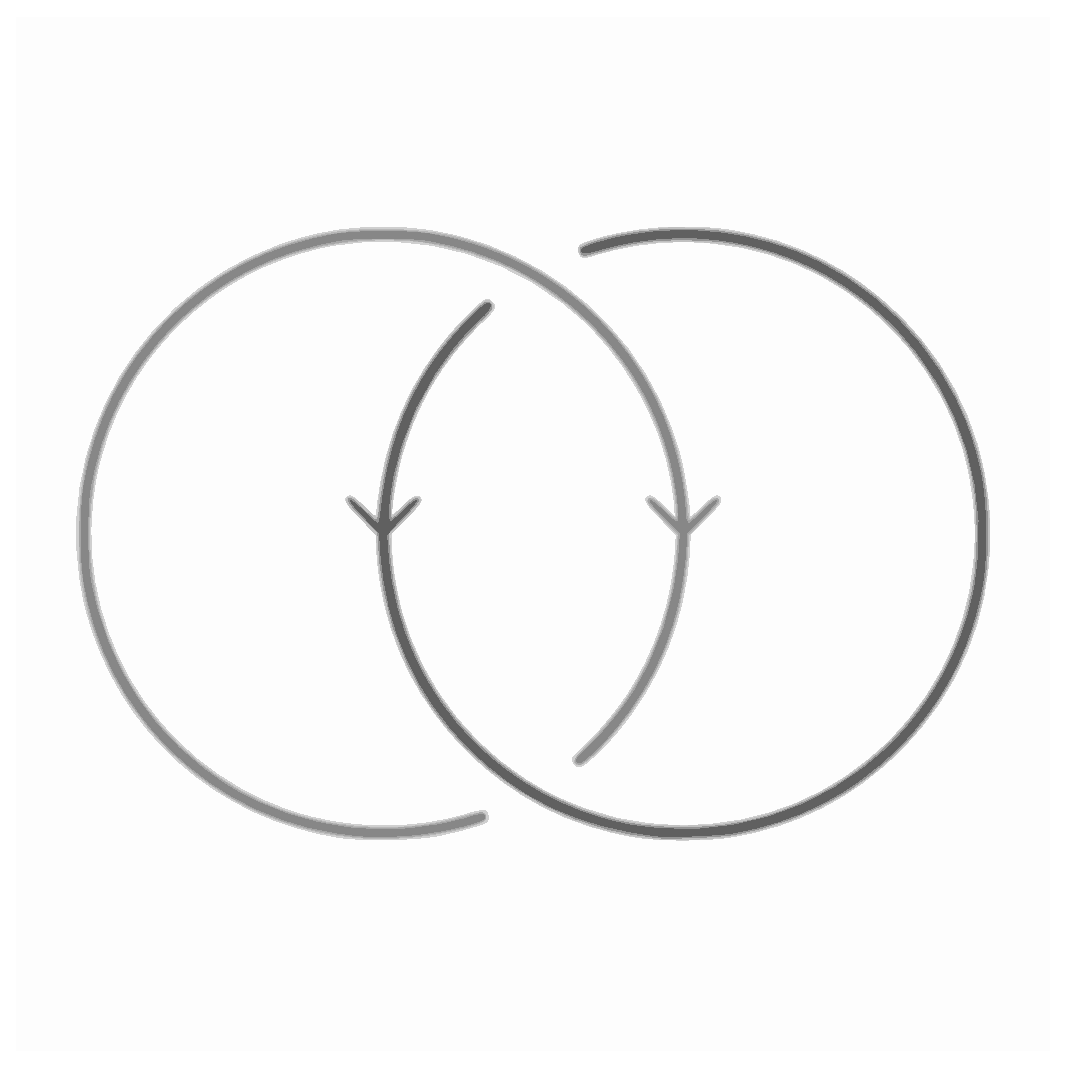
\includegraphics[width= 0.3\textwidth]{hopf}
            \caption{Die Hopf Verschlingung}
            \label{fig:hopf}
        \end{wrapfigure}
        Das trivialste nicht-triviale Beispiel einer Verschlingung mit mehreren Komponenten ist der Hopf Link. Er besteht aus zwei ineinander verschlungenen Unknoten, $L_1, L_2$. Betrachtet man nun zwei Scheiben und verklebt diese mit zwei umgekehrt verdrehten Bändern, so erhält man die Hopf Verschlingung als Rand. Äquivalent möge man sich einen Kreisring $S^1 \times I$ nehmen, der zweifach verdreht ist und beobachtet, dass dieser eine Seifertfläche $S$ darstellt. Das Geschlecht dieser Seifertfläche ist $0$, da es sich um eine Sphäre handelt, aus der zwei offene Scheiben entnommen wurde und somit $\chi_-(S)=0$. Mit anderen Worten ist die obige Bedingung, dass die Thurston-Norm eine Norm ist, nicht erfüllt. Entsprechend existieren Elemente in $H^1(M_L;\RR)$ die sich zu 0 auswerten und durch die Linearität der Thurston-Norm entsteht ein degenerierter Untervektorraum (man überprüft leicht, dass die Fortsetzung nach $\RR$ auch verschwindet). Mit der Subadditivität verschwindet die Thurston-Norm auf dem Vektorraum $H^1(M;\RR)$, also ist die Einheitskugel nicht kompakt, sondern der gesamte Raum. Geht man jedoch zur dualen Norm über, erhält man wieder ein kompaktes Polytop mit ganzzahligen Eckpunkten: 
        \[
              \overline B_{||\cdot||_T^*}= \{\alpha \in H_1(M;\RR)| \sup_{\{\phi \in H^1(M;\RR)\}} \phi(\alpha)\leq 1\}=0
        \] 

        Die folgenden Beispiele sind aus Thurston's Arbeit~\cite{Thurston.1986} entnommen. Die Berechnungen von Thurston bedienen sich lauter Argumente warum keine repräsentierende Fläche existieren kann, die eine geringere Komplexität als die bisher gefundenen hat. Wir werden natürlich unsere Anstrengungen belohnen und Theorem~\ref{thm:haupttheorem} nutzen, um die Thurston-Norm-minimierende Flächen bequemer festzustellen.

        \subsubsection*{Whitehead Verschlingung}

        Die Whitehead Verschlingung ist ein Link der aus zwei Komponenten $L_1,L_2$ besteht. Offensichtlich berandet jede Komponente $L_i$ in $M_{L_i}$ eine Scheibe, die sich in $M_L$ auf eine Kreisscheibe mit zwei entnommenen offenen Scheiben einschränkt (an den Stellen, an denen die offene Tubenumgebung des anderen Knotens die Scheibe durchdringt). Bei diesen Repräsentanten für $l_1$ beziehungsweise $l_2$ berechnet sich die Eulercharakteristik zu $-1$, also gilt $||\pm l_i||_T\leq 1$, offensichtlich gilt aber Gleichheit undin diesem Fall die Thurston-Norm eine tatsächliche Norm. Genauso offensichtlch gilt $||l_1+l_2||_T>0$: die Verschlingungszahl des Whitehead Links ist offensichtlich $0$ (dies sieht man indem man eine Projektion betrachtet in dem die eine Komponente der Unknoten ist), jedoch haben die Randkomponenten jeder Einbettung eines Kreisring $S^1\times I \into S^3$ Verschlingungszahl $\neq 0$ oder sind trivial (durch einen Äquator zu trennen). Also folgt, dass diese Fläche Geschlecht $\ge 1$ hat und somit $2 \leq ||l_1+l_2||_T \leq ||l_1||_T+||l_2||_T =2$ für eine Seifertfläche. Mit Theorem~\ref{thm:haupttheorem} ließe sich diese untere Abschätzung auch mit $\Delta_L = (L_1-1)(L_2-1) = L_1L_2 -L_1-L_2+1$ berechnen, da $\thur {l_1+l_2} \geq \alex {l_1+l_2} \geq (l_1+l_2) (L_1+L_2-0)=2$ Diese ist Seifert-Fläche ergibt sich sogar durch die Seifert-Konstruktion. Folglich:
        \begin{align*}
            ||l_1+l_2||_T =||-(l_1+l_2)||_T &\stackrel * = ||-l_1+l_2||_T = ||l_1-l_2||_T \\
            &=2
        \end{align*}
        wobei die ausgezeichnete Gleichung gilt, da $||-l_1+-l_2||_T\not \in \{0,1\}$ aus obigen Gründen.
        \emph{Behauptung:} Die Thurston-Norm Einheitskugel und ihr Duales sind die Folgenden:\\
        \begin{figure}[H]
        \centering
        \begin{subfigure}[l]{0.4\textwidth}
                \begin{tikzpicture}
            % Axis
            \draw[->] (-3,0)--(3,0) node[below] {$l_1$};
            \draw[->] (0,-3)--(0,3) node[left] {$l_2$};
        
            \draw[] (0,2)--(1,1);
            \draw[] (1,1)--(2,0);
            \draw[] (2,0)--(0,-2);
            \draw[] (0,-2)--(-2,0);
            \draw (-2,0)--(0,2);
        
            \node[below] at (2,0) {$l_2$};
            \node[above right] at (1,1) {$\frac {l_1+l_2}2$};
           % \filldraw[black] (1,1) circle (2pt) node[above right,black] {$\frac {l_1+l_2}2$};
            \foreach \Point in {(0,2), (1,1), (2,0), (0,-2), (-2,0), (0,2), (1,-1), (-1,-1),(-1,1)}{
            \node at \Point {\textbullet};
            }
        
            \end{tikzpicture}
                \caption{$\thurball$}\label{fig:whiteheadthur}
        
        
        \end{subfigure}    
        \hfill
    \begin{subfigure}[r]{0.4\textwidth}
              \begin{tikzpicture}
        % Axis
        \draw[->] (-3,0)--(3,0) node[below] {$L_1$};
        \draw[->] (0,-3)--(0,3) node[left] {$L_2$};

        \draw (-2, -2) --(-2, 0) --(-2, 2) --(0 ,2) --(2 ,2)--(2 ,0)--(2 ,-2) --(0 ,-2) --(-2,-2) ; 
        \foreach \Point in{(-2, -2) ,(-2, 0) ,(-2, 2) ,(0 ,-2) ,(0 ,2) ,(2 ,-2) ,(2 ,0) ,(2 ,2)}{
        \node at \Point {\textbullet};
        }
        \end{tikzpicture}
    \caption{$\dualthurball$}

    \end{subfigure}
    \caption{Einheitskugeln der Whitehead Verschlingung in $H^1(M;\RR)$ und $H_1(M;\RR)$}
    \end{figure}
    Die $8$ berechneten Punkte liegen auf dem Rand von $\thurball$ (die Norm ist stetig), einer konvexen Teilmenge. Es ist eine leichte Übung, dass jede konvexe Teilmenge zweier nächster Punkte in Abbildung~\ref{fig:whiteheadthur} im Rand dieser konvexen Teilmenge enthalten sein muss. Aufgrund der Monotonie folgt die Behauptung für die Einheitskugel. Für die duale Norm, berechnet man entweder $8$ verschiedene Randpunkte, oder beobachtet für jedes $\alpha \in H_1(M;\RR)$ auf welchen Elementen (eine Gerade) $\phi \in H^1(M_L;\RR)$ das Supremum $\phi \alpha$ angenommen wird und sieht direkt das Ergebnis.

    \subsubsection*{Borromäische Ringe}

    Seien $L=L_1 + L_2 + L_3$ die Borromäischen Ringe. Offensichtlich hat jede duale Fläche zu $l_i$, die Komponente $L_i$ als Rand, (sonst wäre der Meridian aufgrund eines Schnittzahlenarguments im Kern von $l_i$). Folglich hat also jede Fläche dual zu $l_i$ mindestens 3 Randkomponenten. Da eine Sphäre mit 3 entnommenen offenen Scheiben (also eine abgeschlossene Scheibe mit 2 Durchlöcherungen), wobei die eine Randkomponente aufgespannt wird von der entnommenen Komponente $\nu(L_i)$, bereits dual zu $l_i$ ist gilt wieder $\thur {\pm l_i}=1$ für jedes $i$. Ähnlich wie beim letzten Beispiel der Whitehead Verschlingungen, möchten wir nun --- in Dimension 3 --- die berandenden Seiten der Einheitskugel durch Berechnung einiger Punkte feststellen und sie dadurch bestimmen. Es berechnet sich $\Delta_L = L_1L_2L_3 -\sum L_iL_j + \sum L_i -1$ und somit folgt leicht die Alexander-Norm einer beliebigen Kohomologieklasse, insbesondere:
    \[
        3= \alex {\pm l_1 \pm l_2 \pm l_3} \leq \thur {\pm l_1 \pm l_2 \pm l_3} \leq  \thur {l_1} + \thur {l_2} + \thur{l_3}=3
    \]

    Wegen $\thur {\pm l_i} = 1$  und $\thur {\frac13(\pm l_1 \pm l_2 \pm l_3)}=1$ folgt dass die Randseiten der Einheitskugel, die Standard-2-Simplices sind, die von den Einheitsvektoren aufgespannt werden. Somit berechnet sich $\thurball$ zu einem Oktahedron, siehe Abbildung~\ref{fig:borromthur}. Mit derselben Überlegung wie im vorhergehenden Beispiel, erkennt man strahlenweise die Form von $\dualthurball$ als Würfel.

\begin{figure}
\centering
    \begin{subfigure}{0.4\textwidth}
    
        \tdplotsetmaincoords{70}{110}        
        \begin{tikzpicture}[tdplot_main_coords]

        \draw[dashed] (-2,0,0) -- (2,0,0) ;
        \draw[dashed] (0,-2,0) -- (0,2,0) ;
        \draw[dashed] (0,0,-2) -- (0,0,2); 
        \draw[->] (2,0,0) -- (3,0,0) node[anchor=north east]{$l_1$};
        \draw[->] (0,2,0) -- (0,3,0) node[anchor=north west]{$l_2$};
        \draw[->] (0,0,2) -- (0,0,3) node[anchor=south]{$l_3$};
    
    
        \foreach \x in {2,-2}{
                \node at (\x  ,0,0) {\textbullet};
                \node at (0,\x ,0) {\textbullet};
                \node at (0,0,\x ) {\textbullet};
                \draw (\x,0,0)--(0,\x,0);
                \draw (\x,0,0) -- (0,0,\x);
                \draw (\x,0,0)--(0,-\x,0);
                \draw (\x,0,0) -- (0,0,-\x);
                \draw (0,\x,0) -- (0,0,\x);
                \draw (0,\x,0) -- (0,0,-\x);
                }
            \draw [fill,opacity=0.3] (2,0,0) -- (0,2,0) -- (0,0,2) -- cycle;
         %   \draw[thick] (2/3-0.3,2/3,2/3) -- (2/3+0.3,2/3,2/3);
       %     \draw[thick] (2/3,2/3-0.2,2/3) -- (2/3,2/3+0.2,2/3);
         %   \draw[thick] (2/3,2/3,2/3-0.2) -- (2/3,2/3,2/3+0.2);
         %   \node[above] at (2/3+0.2,2/3,2/3+0.2) {$l/3$};
        \end{tikzpicture}
        \caption{$\thurball$}\label{fig:borromthur}
    \end{subfigure}
    \hfill
    \begin{subfigure}[r]{0.4\textwidth}
    
        \tdplotsetmaincoords{70}{110}
        \begin{tikzpicture}[tdplot_main_coords]

        \draw[dashed] (-2,0,0) -- (2,0,0) ;
        \draw[dashed] (0,-2,0) -- (0,2,0) ;
        \draw[dashed] (0,0,-2) -- (0,0,2); 
        \draw[->] (2,0,0) -- (3,0,0) node[anchor=north east]{$l_1$};
        \draw[->] (0,2,0) -- (0,3,0) node[anchor=north west]{$l_2$};
        \draw[->] (0,0,2) -- (0,0,3) node[anchor=south]{$l_3$};
    
        \foreach \x in {2,-2}{
                \node at (\x  ,0,0) {\textbullet};
                \node at (0,\x ,0) {\textbullet};
                \node at (0,0,\x ) {\textbullet};
                }
        \foreach \x in {2,-2}{
            \foreach \y in {2,-2}{
            \foreach \z in {2,-2}{
            \draw (\x,\y,\z) -- (\x,\y,-\z);
            \draw (\x,\y,\z) -- (-\x,\y,\z);
            \draw (\x,\y,\z) -- (\x,-\y,\z);
            }
            }
        }
        \end{tikzpicture}
        \caption{$\dualthurball$}
    \end{subfigure}
    \caption{Die Einheitskugeln der Borromäischen Ringe}
\end{figure}

%!TEX root = main.tex

\section{Persönliche Notizen während der Erstellung}
	Sei $m(G)/m(\ker \phi)m(G)$ die algebraische Beschreibung des Alexander Moduls als $\ZZ[F]=\ZZ[G]/m(\ker \phi)$-Modul. Dann dieser Quotient endl erz denn

	Alex und Thurston Norm sind wirklich Normen 

	Warum nimmt Mcmullen die Homologie relativ allen Lifts vom Basispunkt?  !!

	Einschränkung: Mannigfaltigkeit glatt?

	Im Beweis wo $b_1(G)=1$ gezeigt wird, ist es nicht auch möglich, die Argumentation über die Fundamentalgruppe wegzulassen und stattdessen zu zeigen:
	\begin{itemize}
		\item G ist zsh
		\item $\delta_+(M_i) = \delta_-(M_i)=1 \implies G$ ist Mannigfaltigkeit
		\item $G$ ist kompakt
	\end{itemize}
	$\implies$ mit Klassifikation von 1-Mft ist $G$ ein Kreis.

	Andersrum: wenn $G$ vom Homotopietyp ein Kreis ist (also zsh und $\pi_1=\ZZ$), dann kann nur noch $\delta_\pm(M_i)=0$ passieren

	Eigenschaften der Tnorm : $kerx$ ist ein linearer Unterraum. und x $x$ ist auf den Nebenklassen von kerx konstant! und 1-ball

	zweiseitiger KRagen

	noch uct erwähnen

	obda fibration indivisible (flp.pdf)


	vielleicht noch Knoten: duale Fläche als Urbild ist Seifertfläche
	bis jetzt nur: Seifertfläche => dual


	fragen an Fr Hamenstädt
	\begin{itemize}
		\item CW endlich Struktur (Kpt argument oder Morse Argument)
		\item  berandende Fläche nullhomolog wenn mehr Radkomponenten
		\item 
	\end{itemize}

	{Strukturelles}
	\begin{itemize}
		\item Algebra evtl nach vorne damit man es benutzen kann
		\item Examples komplett umstrukturieren mit Unterkapiteln
	\end{itemize}
%maybe Appendix: Algebraische Sichweise 

\listoftodos

\bibliography{ref}
\bibliographystyle{plain}

\end{document}
